\textbf{1.1.1.} 电荷量分别为 $q_{1}$ 和 $q_{2}$ 的两个静止的点电荷，相距为 $r$ ，试求下列情况下它们之间的相互作用力，即 $q_{1}$ 作用在 $q_{2}$ 上的力 $\mathbf{F}_{21}$ 和 $q_{2}$ 作用在 $q_{1}$ 上的力 $\mathbf{F}_{12}$ :(1) $q_{1}$ 和 $q_{2}$ 都在真空中；(2) $q_{1}$ 和 $q_{2}$ 都在均匀介质中；(3) $q_{2}$ 在导体空腔内， $q_{1}$ 则在导体外.

\vfill

\textbf{1.1.2.} 有两个静止的点电荷, 它们的电荷量都是 1C, 试分别求它们相距为 1m 和 1km 时, 它们之间相互作用力的大小.

\vfill

\newpage

\textbf{1.1.3.} 铁原子核里两质子相距为 $4.0 \times 10^{-15} \mathrm{~m}$ , 每个质子的电荷量都是 1.6 $\times 10^{-19} \mathrm{C}$ . 实验证明, 库仑定律在这个距离上仍然成立. 试求这两个质子间库仑力的大小.

\vfill

\textbf{1.1.4.} 真空中两个点电荷静止时相距 10cm, 它们间的相互作用力为 $9.0 \times 10^{-4} ~N$ ; 当它们合在一起时, 就成为 $3.0 \times 10^{-8} ~C$ 的一个点电荷. 试问原来两电荷的电荷量各是多少?

\vfill

\newpage

\textbf{1.1.5.} 质量都是 m 的两小球, 带有相同的电荷量 q, 用长度都是 l 的细丝线挂在同一点, 静止时两线夹角为 $2\theta$ [图 1.1.5(1)]. 设小球的半径和线的质量都可略去不计, 试求 q 的值.

\vfill

\textbf{1.1.6.} A、B 两个带电小球，所带电荷量都是 q，用等长的两根丝线悬于同一点，线长为 l, B 球靠在绝缘墙上，它的悬线竖直，如图 1.1.6(1) 所示。当 A 球的质量为 m 时，因静电斥力使两球相距为 x，达到静止。试问在 A、B 两球所带电荷量不变的情况下，A 球的质量增为多大时，A、B 间的静止距离缩短为 x/2？设小球的半径和丝线的质量都可略去不计。

图1.1.6(1)

图1.1.6(2)
\begin{center}
    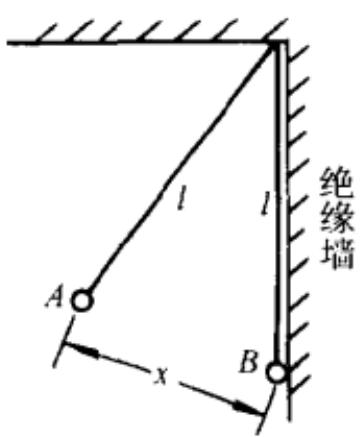
\includegraphics[width=0.5\linewidth]{figures/fig_1_1_6_1.jpg}
\end{center}
\begin{center}
    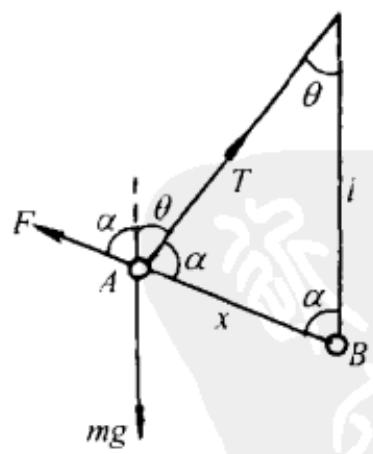
\includegraphics[width=0.5\linewidth]{figures/fig_1_1_6_2.jpg}
\end{center}

\vfill

\newpage

\textbf{1.1.7.} 两个固定的点电荷,电荷量分别为 q 和 4q,相距为 l.(1)试问在什么地方放一个什么样的点电荷,可以使这三个电荷都达到平衡(即每个电荷受另外两个电荷的库仑力之和都等于零)?(2)这种平衡是稳定平衡还是不稳定平衡?

图1.1.7
\begin{center}
    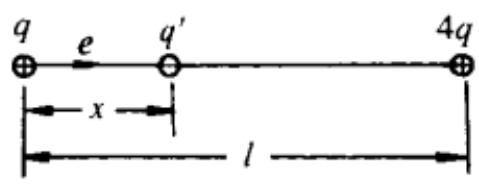
\includegraphics[width=0.5\linewidth]{figures/fig_1_1_7.jpg}
\end{center}

\vfill

\textbf{1.1.8.} 电荷量都是 $q$ 的三个点电荷, 分别放在正三角形的三个顶点. 试问: (1) 在这三角形中心放一个什么样的点电荷, 就可以使这四个电荷都达到平衡 (即每个电荷受其他三个电荷的库仑力之和均为零)? (2) 这种平衡与三角形的边长有无关系? (3) 这样的平衡是稳定平衡还是不稳定平衡?

\vfill

\newpage

\textbf{1.1.9.} 电荷量都是 $q = 1.6 \times 10^{-19} \mathrm{C}$ 的三个点电荷, 分别固定在边长为 $a = 3.0 \times 10^{-10} \mathrm{~m}$ 的正三角形的三个顶点; 在这三角形的中心 $O$ , 有一个质量为 $m = 2.3 \times 10^{-26} \mathrm{~kg}$ 、电荷量为 $Q = -4.8 \times 10^{-19} \mathrm{C}$ 的粒子。(1)试论证这个粒子处在平衡位置; (2)设这粒子以 $O$ 为中心, 沿垂直于三角形平面的轴线作微小振动, 试求振动频率.

图1.1.9
\begin{center}
    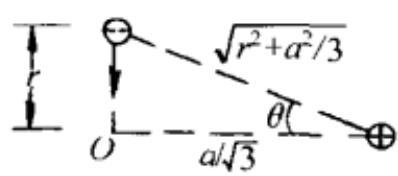
\includegraphics[width=0.5\linewidth]{figures/fig_1_1_9.jpg}
\end{center}

\vfill

\textbf{1.1.10.} 电荷量都是 q 的四个点电荷, 分别处在正方形的四个顶点, 如图 1.1.10(1) 所示。(1) 在这正方形中心放一个什么样的点电荷, 就可以使每个电荷都达到平衡? (2) 这样的平衡是稳定平衡还是不稳定平衡?

\vfill

\newpage

\textbf{1.1.11.} 两个固定的点电荷, 电荷量都是 $Q$ , 相距为 $l$ , 联线中点为 $O$ ; 另一点电荷, 电荷量为 $q$ , 在联线的中垂面上距离 $O$ 为 $r$ 处, 如图 1.1.11 所示. (1) 求 $q$ 受的力; (2) 若开始时 $q$ 是静止的, 然后让它自己运动, 问它将如何运

图1.1.11

动？试分别就 q 与 Q 同号和异号两种情况加以讨论.
\begin{center}
    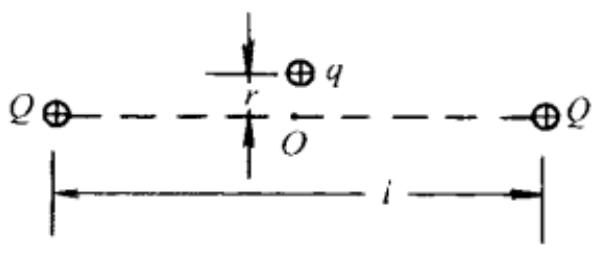
\includegraphics[width=0.5\linewidth]{figures/fig_1_1_11.jpg}
\end{center}

\vfill

\textbf{1.1.12.} 卢瑟福实验证明: 当两个原子核之间的距离小到 $10^{-15}$ m 时, 它们之间的排斥力仍遵守库仑定律. 金的原子核中有 79 个质子, 氦的原子核(即 $\alpha$ 粒子)

中有2个质子.已知每个质子的电荷量为 $1.60\times10^{-19}C,\alpha$ 粒子的质量为 $6.68\times10^{-27}kg$ .当 $\alpha$ 粒子与金核相距为 $6.9\times10^{-15}m$ 时,设它们都可当作点电荷,试求金核作用在 $\alpha$ 粒子上的库仑力和 $\alpha$ 粒子因此而产生的加速度.

\vfill

\newpage

\textbf{1.1.14.} 氢原子由一个质子(即氢原子核)和一个电子组成. 根据经典模型, 在正常状态下,电子绕核作圆周运动,轨道半径是 $5.29\times10^{-11}m$ .已知电子带负电,质子带正电,它们的电荷量大小相等,都是 $1.60\times10^{-19}C$ ,电子质量 $m=9.11\times10^{-31}kg$ ,质子质量 $M=1.67\times10^{-27}kg$ ,万有引力常数 $G=6.67\times10^{-11}m^{3}/kg\cdot s^{-2}$ .试求:(1)电子受质子作用的库仑力;(2)电子受质子作用的库仑力是万有引力的多少倍?(3)电子绕核运动的速率和频率.

\vfill

\textbf{1.1.15.} 氢原子由一个质子(即氢原子核)和一个电子组成.根据经典模型,电子环绕质子作圆周运动.假定电子环绕质子运动的角动量只能是 $\hbar = 1.054 \times 10^{-34} J \cdot s$ 的整数倍,即 $mr^{2}\omega = n\hbar, n = 1, 2, 3, \cdots$ .已知质子带正电,电子带负电,它们的电荷量的大小都是 $1.602 \times 10^{-19} C$ ,电子质量为 $9.11 \times 10^{-31} 千克$ .试求 n = 1(基态)时电子轨道半径的值(这个值通常称为玻尔半径).

\vfill

\newpage

\textbf{1.1.16.} 真空中有一固定的点电荷, 其电荷量为 $Q$ ; 另一质量为 $m$ 、电荷量为 $q$ 的质点, 因 $qQ < 0$ , 它们之间的库仑力是吸引力. 在这力的作用下, $m$ 绕 $Q$ 作匀速圆周运动, 半径为 $r$ , 周期为 $T$ . 试证:

$$
r ^ {3} / T ^ {2} = - q Q / 1 6 \pi^ {3} \varepsilon_ {0} m
$$

\vfill

\textbf{1.1.17.} 真空中有一固定的点电荷, 其电荷量为 $Q$ ; 另一质量为 $m$ 、电荷量为 $q$ 的质点, 因 $qQ < 0, q$ 与 $Q$ 间的库仑力是吸引力. 试证明, 在这力的作用下, $m$ 的轨迹是以 $Q$ 为焦点的圆锥曲线.

图1.1.17
\begin{center}
    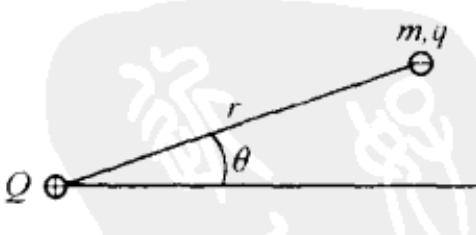
\includegraphics[width=0.5\linewidth]{figures/fig_1_1_17.jpg}
\end{center}

\vfill

\newpage

\textbf{1.1.18.} 把总电荷量为 $Q$ 的同一种电荷分成两部分，一部分均匀分布在地球上，另一部分均匀分布在月球上，使它们之间的库仑力正好抵消万有引力。已知 $\frac{1}{4\pi\varepsilon_0} = 8.99\times 10^{9}\mathrm{Nm}^{2} / \mathrm{C}^{2}$ ，万有引力常量 $G = 6.67\times 10^{-11}\mathrm{Nm}^2 /\mathrm{kg}^2$ ，地球质量 $M$ $= 5.98\times 10^{24}\mathrm{kg}$ ，月球质量 $m = 7.34\times 10^{22}\mathrm{kg}$ (1)试求 $Q$ 的最小值；(2)如果电荷量的分配与质量成正比，试求 $Q$ 的值。

\vfill

\textbf{1.1.19.} 电荷量 Q 均匀分布在半径为 R 的金属圆环上, 现在环中心放一个电荷量为 q 的点电荷. 试求由于 q 的出现而在环中产生的张力.

\vfill

\newpage

\textbf{1.1.20.} 电荷量 q 均匀分布在半径为 R 的圆环上, 在环的轴线上有一条均匀带电的直线, 单位长度的电荷量为 $\lambda$ , 直线的一端在环心, 另一端趋向无穷远. 试求它们之间的相互作用力.

\vfill

\textbf{1.2.1.} 电场强度的物理意义是单位正电荷量所受的力. 因为电荷量的单位是库仑, 故某点的电场强度等于在该点放一个电荷量为一库仑的点电荷所受的力. 你认为对吗?

\vfill

\newpage

\textbf{1.2.2.} 氢原子由一个质子(氢原子核)和一个电子组成. 根据经典模型, 在正常状态下, 电子绕核作匀速圆周运动, 轨道半径是 $5.29 \times 10^{-11} \mathrm{~m}$ . 已知质子的电荷量为 $1.60 \times 10^{-19} \mathrm{C}$ , 试求质子在电子轨道上产生的电场强度的大小.

\vfill

\textbf{1.2.3.} 两个点电荷, 电荷量分别为 $q_{1} = 8.0\mu \mathrm{C}$ , $q_{2} = -16.0\mu \mathrm{C}$ , 相距 $20\mathrm{cm}$ . 试求这两个电荷在离它们都是 $20\mathrm{cm}$ 处产生的电场强度 $\pmb{E}$ .

\vfill

\newpage

\textbf{1.2.4.} 电荷量都是 q 的两个点电荷, 相距为 l, 联线的中点为 O. 试求它们在联线的中垂面上离 O 为 r 处产生的电场强度.

\vfill

\textbf{1.2.5.} 相距为 $l$ 的两个点电荷, 电荷量分别为 $q$ 和 $-q$ , 它们间联线的中点为 $O$ , 如图 1.2.5(1) 所示. (1) 试求它们在下列两处所产生的电场强度; (i) 在联线的延长线上离 O 为 r 处；(ii) 在联线的中垂面上离 O 为 r 处。(2) 对于 $r \gg l$ 的区域来说，这两个电荷构成的系统称为电偶极子。试求电偶极子在上述两处产生的电场强度。

图1.2.5(1)

图1.2.5(2)
\begin{center}
    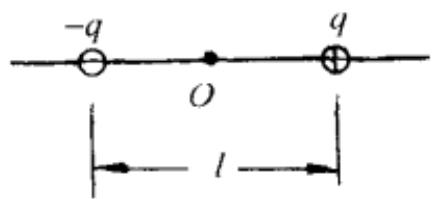
\includegraphics[width=0.5\linewidth]{figures/fig_1_2_5_1.jpg}
\end{center}
\begin{center}
    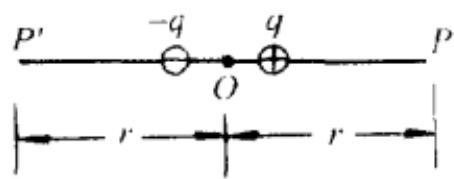
\includegraphics[width=0.5\linewidth]{figures/fig_1_2_5_2.jpg}
\end{center}

\vfill

\newpage

\textbf{1.2.6.} 相距为 $l$ 的两个点电荷, 电荷量分别为 $q$ 和 $-q$ , 它们联线的中点为 $O$ , 如图 1.2.6(1) 所示. $e$ 是从 $-q$ 到 $q$ 方向上的单位矢量, $r$ 是 $O$ 到 $P$ 点的位矢, $\theta$ 是 $r$ 与 $l$ 的夹角. (1) 试求它们在 $P$ 点产生的电场强度 $E$ 在 $r$ 方向上的分量 $E_r$ 和在 $\theta$ 方向上的分量 $E_\theta$ . (2) 对于 $r \gg l$ 的区域来说, 这两个电荷构成的系统称为电偶极子. 试求电偶极子在 $P$ 点产生的 $E_r$ 和 $E_\theta$ .

图1.2.6(1)

图1.2.6(2)
\begin{center}
    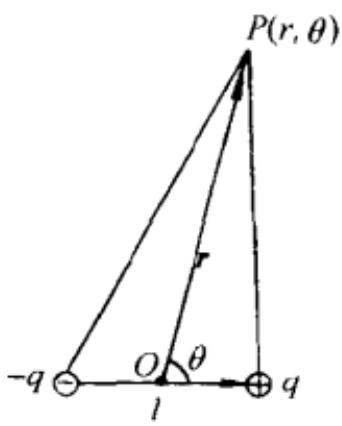
\includegraphics[width=0.5\linewidth]{figures/fig_1_2_6_1.jpg}
\end{center}
\begin{center}
    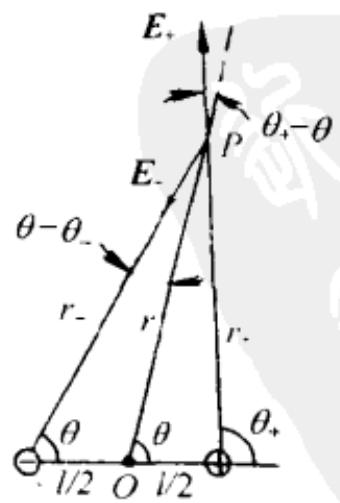
\includegraphics[width=0.5\linewidth]{figures/fig_1_2_6_2.jpg}
\end{center}

\vfill

\textbf{1.2.7.} 相距为 $l$ 的两个点电荷, 电荷量分别为 $q$ 和 $-q$ , 以它们的联线为 $x$ 轴, 联线的中点为原点, 取笛卡儿坐标系如图 1.2.7(1) 所示. (1) $P(x, y)$ 为 $x, y$ 平面上任一点, 试求它们在 $P$ 点产生的电场强度 $\pmb{E}$ ; (2) 对于 $r \gg l$ 的区域来说, 这两个电荷构成的系统称为电偶极子. 试求电偶极子在 $P$ 点产生的电场强度.

图1.2.7(1)

图1.2.7(2)
\begin{center}
    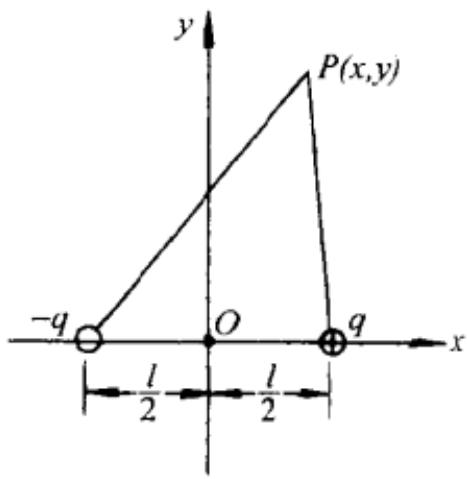
\includegraphics[width=0.5\linewidth]{figures/fig_1_2_7_1.jpg}
\end{center}
\begin{center}
    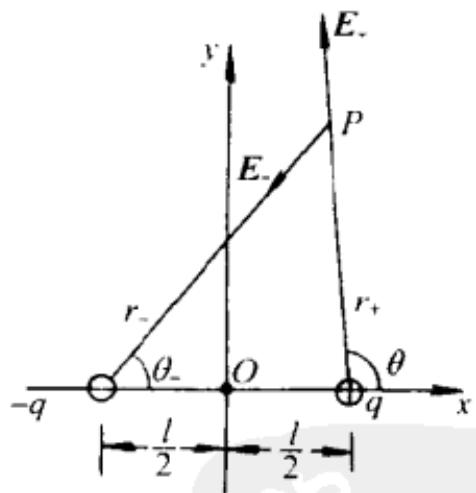
\includegraphics[width=0.5\linewidth]{figures/fig_1_2_7_2.jpg}
\end{center}

\vfill

\newpage

\textbf{1.2.8.} 一电偶极子的电偶极矩为 $p = ql$ ，以它的中心 $O$ 为原点，沿 $l$ 取极轴或 $x$ 轴，如图1.2.8(1)所示。 $P$ 为空间任一点，其位矢为 $r$ 。以 $l$ 和 $r$ 构成的平面为 $x - y$ 平面。试证明： $p$ 在 $P$ 点产生的电场强度 $E$ ，(1)用极坐标表示为

$$
\boldsymbol {E} = \frac {1}{4 \pi \varepsilon_ {0} r ^ {3}} \left[ \frac {3 (\boldsymbol {p} \cdot \boldsymbol {r})}{r ^ {2}} \boldsymbol {r} - \boldsymbol {p} \right]
$$

(2)用笛卡儿坐标表示为

$$
\boldsymbol {E} = \frac {p}{4 \pi \varepsilon_ {0} (x ^ {2} + y ^ {2}) ^ {5 / 2}} [ (2 x ^ {2} - y ^ {2}) i + 3 x y j ]
$$

图1.2.8(1)

图1.2.8(2)
\begin{center}
    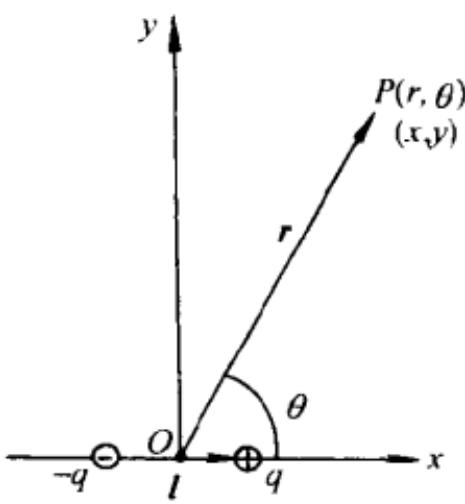
\includegraphics[width=0.5\linewidth]{figures/fig_1_2_8_1.jpg}
\end{center}
\begin{center}
    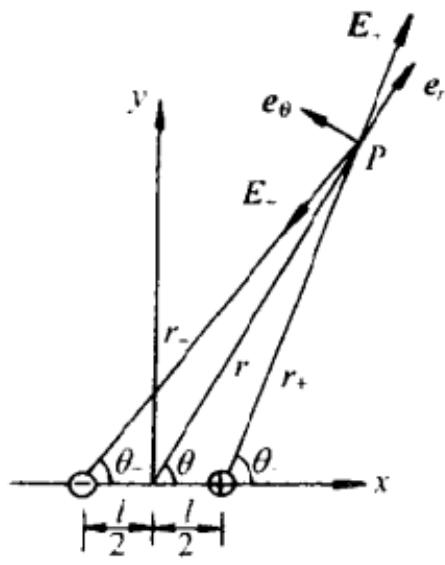
\includegraphics[width=0.5\linewidth]{figures/fig_1_2_8_2.jpg}
\end{center}

\vfill

\textbf{1.2.9.} 如图 1.2.9, p 是一电偶极子的电偶极矩. 试证明: 在 $\theta = \arccos\left(\frac{1}{\sqrt{3}}\right)$ 处, p 所产生的电场强度 E 与 p 垂直.

\vfill

\newpage

\textbf{1.2.10.} 电荷量都是 q 的两个点电荷, 相距为 2l, 另一点电荷的电荷量为

图1.2.10

-2q,处在它们联线的中点,如图1.2.10所示. $P$ 是它们延长线上的一点， $P$ 到 $-2q$ 的距离为 $r$ . (1)试求这三个点电荷在 $P$ 点产生的电场强度；(2)对于 $r \gg l$ 的区域来说，这个电荷系统称为线性电四极子.试求这线性电四极子在 $P$ 点产生的电场强度.
\begin{center}
    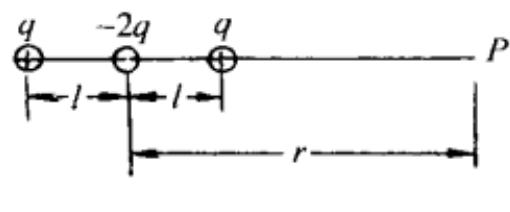
\includegraphics[width=0.5\linewidth]{figures/fig_1_2_10.jpg}
\end{center}

\vfill

\textbf{1.2.11.} 四个点电荷分别处在一个边长为 $l$ 的正方形的四个角上，它们的电荷量分别为 $-q, q, -q$ 和 $q$ ，如图1.2.11(1)所示。 $P$ 是与正方形在同一平面内的一点， $P$ 到正方形中心 $O$ 的距离为 $r$ ，且 $OP$ 联线平行于正方形的两边。(1)试求四个电荷在 $P$ 点产生的电场强度；(2)对于 $r \gg l$ 的区域来说，这四个电荷构成

图1.2.11(1)

的系统称为平面电四极子. 试求这平面电四极子在 $P$ 点产生的电场强度.
\begin{center}
    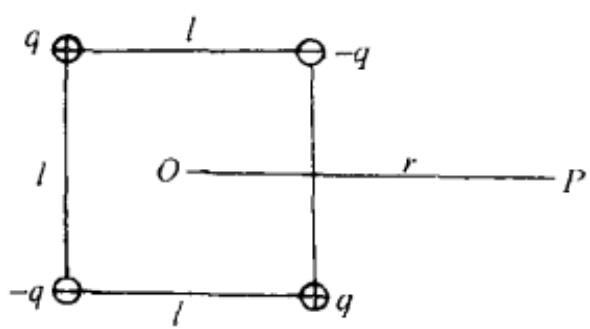
\includegraphics[width=0.5\linewidth]{figures/fig_1_2_11.jpg}
\end{center}

\vfill

\newpage

\textbf{1.2.12.} 电荷量 q 均匀地分布在长为 2l 的一段直线上，线的中点为 O。试求这电荷在下列各处产生的电场强度：(1) 线的延长线上离 O 为 r 处；(2) 线的中垂面上离 O 为 r 处；(3) 通过一端的垂面上离该端为 r 处。

图1.2.12(1)
\begin{center}
    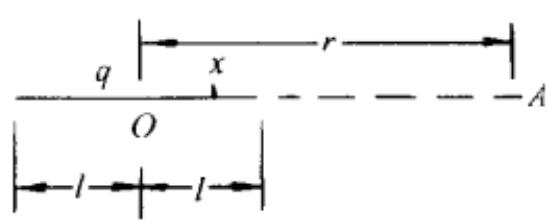
\includegraphics[width=0.5\linewidth]{figures/fig_1_2_12.jpg}
\end{center}

\vfill

\textbf{1.2.14.} 半无限长的直线均匀带电,单位长度的电荷量为 $\lambda$ . 试证明:端垂面(即过端点并与这直线垂直的平面)上除端点外,其他任何一点,电场强度 E 的方向都与这直线成 $45^{\circ}$ 角.

\vfill

\newpage

\textbf{1.2.15.} 电荷量 q 均匀分布在边长为 l 的正方形的四边上。(1)试求这正方形轴线上离中心为 r 处的电场强度 E；(2)试证明：在 $r \gg l$ 处，E 相当于 q 集中在正方形中心所产生的电场强度.

\vfill

\textbf{1.2.16.} 电荷量 q 均匀分布在半径为 R 的圆环上。(1)试求这电荷在轴线上离环心为 r 处的电场强度 E;(2)画出 E-r 曲线(即以 r 为横坐标,以 E 的大小 E 为纵坐标的 E 与 r 的关系曲线);(3)轴线上什么地方 E 最大? 其值是多少?(4)

图1.2.16(1)

试证明: 当 $r \gg R$ 时, E 趋于 q 集中在环心所产生的电场强度.
\begin{center}
    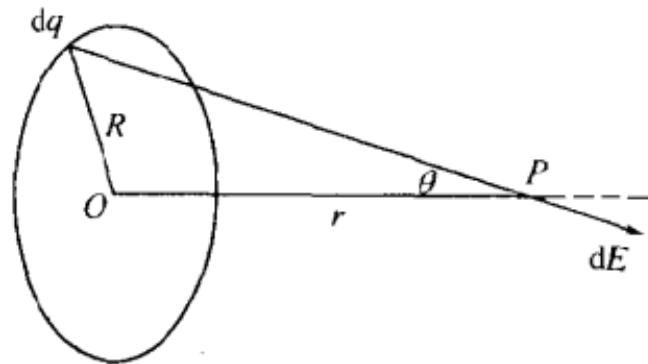
\includegraphics[width=0.5\linewidth]{figures/fig_1_2_16.jpg}
\end{center}

\vfill

\newpage

\textbf{1.2.17.} 两个共轴的均匀带电圆环, 半径都是 R, 相距为 l, 所带电荷量分别为 q 和 -q; 以两环间轴线的中点 O 为原点, 沿轴线取 x 轴, 如图 1.2.17 所示. 已知 $l \ll R$ , 试求轴线上 x 处的电场强度.

图1.2.17
\begin{center}
    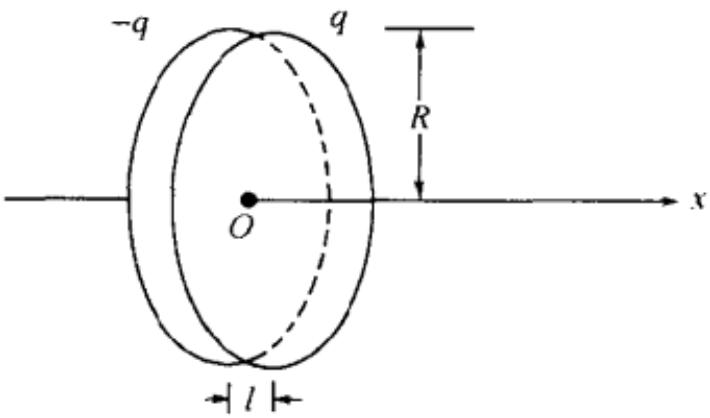
\includegraphics[width=0.5\linewidth]{figures/fig_1_2_17.jpg}
\end{center}

\vfill

\textbf{1.2.18.} 电荷量 q 均匀分布在半径为 R 的半圆环上, 试求环心的电场强度.

\vfill

\newpage

\textbf{1.2.19.} 电荷分布在半圆环 $ABC$ 上, 单位长度的电荷量为 $\lambda = \lambda_0\sin \theta$ , 式中 $\lambda_0$ 为常量, $\theta$ 为通过环两端 $A, C$ 的直径与环的半径 $OB$ 之间的夹角, 如图1.2.19(1)所示. 试证明: 环上的电荷在直径 $AC$ 上任何一点产生的电场强度 $E$ 都与直径 $AC$ 垂直.

图1.2.19(1)

图1.2.19(2)
\begin{center}
    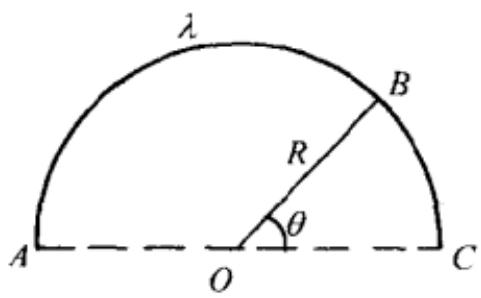
\includegraphics[width=0.5\linewidth]{figures/fig_1_2_19_1.jpg}
\end{center}
\begin{center}
    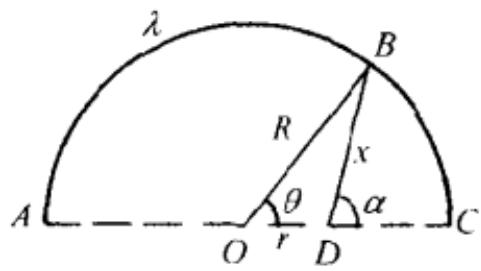
\includegraphics[width=0.5\linewidth]{figures/fig_1_2_19_2.jpg}
\end{center}

\vfill

\textbf{1.2.20.} 一无穷长均匀带电线,有一部分弯成半圆形,其余部分则为两条无穷长的平行直线,两直线都与半圆的直径 AB 垂直,且它们都在同一平面内,如图 1.2.20(1) 所示.试求圆心 O 的电场强度.

\vfill

\newpage

\textbf{1.2.21.} 半径为 R 的圆面均匀带电, 电荷量的面密度为 $\sigma$ . (1) 试求这圆面电荷在轴线上离圆心为 r 处产生的电场强度 E; (2) 在保持 $\sigma$ 不变的情况下, 当 $R \to 0$ 和 $R \to \infty$ 时结果各如何? (3) 在保持总电荷量 $Q = \pi R^{2} \sigma$ 不变的情况下, 当 $R \to 0$ 和 $R \to \infty$ 时结果各如何?
\begin{center}
    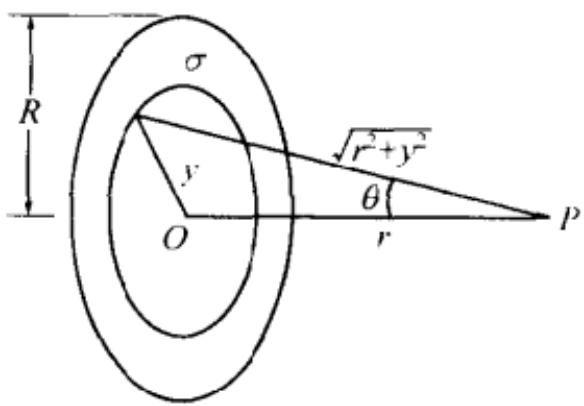
\includegraphics[width=0.5\linewidth]{figures/fig_1_2_21.jpg}
\end{center}

\vfill

\textbf{1.2.22.} 两个共轴线的圆面, 半径都是 R, 相距为 l, 它们上面都均匀分布着电荷, 电荷量的面密度分别为 $\sigma$ 和 $-\sigma$ ; 以它们间轴线的中点 O 为原点, 沿轴线取 x 轴, 如图 1.2.22(1) 和图 1.2.22(2) 所示. 已知 $l \ll R$ , 试求轴线上 x 处的电场强度.

\vfill

\newpage

\textbf{1.2.23.} 一无限大平面均匀带电,电荷量的面密度为 $\sigma$ ,但这面上有一半径为 $R$ 的圆洞.试求这圆洞轴线上离洞心为 $r$ 处的电场强度.

\vfill

\textbf{1.2.24.} 一无限大平面均匀带电,电荷量的面密度为 $\sigma$ ,它所产生的电场强度的大小为 $\frac{\sigma}{2\varepsilon_0}$ .试证明:在离该面为 $r$ 处的 $P$ 点(图1.2.24),电场强度有一半是到 $P$ 的距离为 $2r$ 以内的电荷产生的.

\vfill

\newpage

\textbf{1.2.25.} 电荷量 q 均匀分布在半径为 R 的球面上, 试求距离球心为 r 处的电场强度: (1) r < R; (2) r > R.

图1.2.25(1)
\begin{center}
    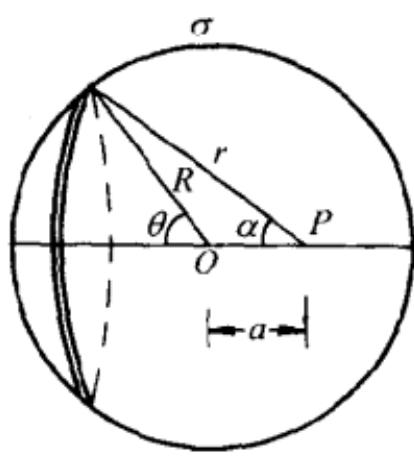
\includegraphics[width=0.5\linewidth]{figures/fig_1_2_25.jpg}
\end{center}

\vfill

\textbf{1.2.26.} 电荷量 q 均匀分布在半径为 R 的球面上, 试求这球面上电荷所在处的电场强度.

\vfill

\newpage

\textbf{1.2.27.} 电荷量 Q 均匀分布在半径为 R 的球面上, 试求这球面由于电荷而产生的张力系数 $\alpha$ .

\vfill

\textbf{1.2.28.} 电荷分布在半径为 R 的球面上, 电荷量的面密度为 $\sigma = a \cdot R$ , 式中 a 是一个常矢量, R 是球心到球面上一点的矢径. 试求球心的电场强度.

\vfill

\newpage

\textbf{1.2.29.} 电荷分布在半径为 R 的球面上, 电荷量的面密度为 $\sigma = a \cdot R$ , 式中

图1.2.29(1)

a 是一个常矢量，R 是球心到球面上一点的矢径. 试证明：球内电场是均匀电场.
\begin{center}
    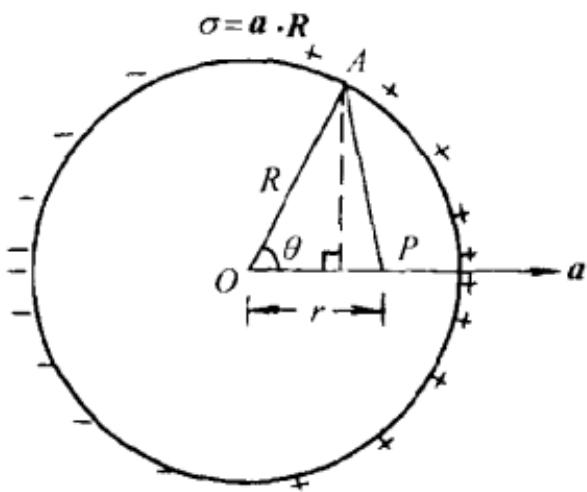
\includegraphics[width=0.5\linewidth]{figures/fig_1_2_29.jpg}
\end{center}

\vfill

\textbf{1.2.30.} 电荷量 q 均匀分布在半径为 R 的球冠(球缺)面上, 球冠边缘对球心 O 的张角为 $2\theta$ , 如图 1.2.30(1) 所示. 试求这电荷在球心产生的电场强度.

图1.2.30(1)

图1.2.30(2)
\begin{center}
    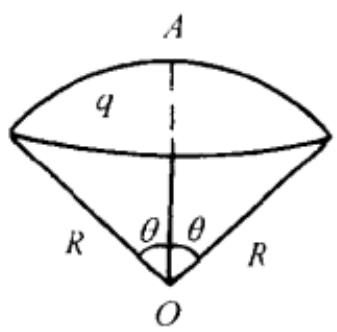
\includegraphics[width=0.5\linewidth]{figures/fig_1_2_30_1.jpg}
\end{center}
\begin{center}
    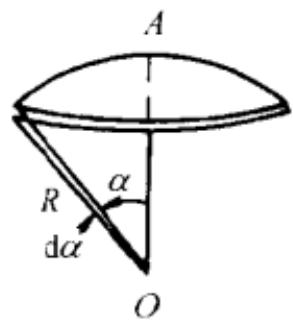
\includegraphics[width=0.5\linewidth]{figures/fig_1_2_30_2.jpg}
\end{center}

\vfill

\newpage

\textbf{1.2.31.} 电荷分布在一无穷长的圆柱面上, 电荷量的面密度为 $\sigma = \sigma_0\cos \phi$ , 式中 $\sigma_0$ 是常量, $\phi$ 是圆柱横截面内, 半径 $OC$ 与直径 $AOB$ 的夹角, 如图 1.2.31 所示. 试求圆柱轴线上 $O$ 点的电场强度.

\vfill

\textbf{1.2.32.} 电荷分布在半径为 R 的球体内, 电荷量的密度为 $\rho = a \cdot r$ , 式中 a 是

图1.2.32

常矢量，r 是从球心到球内一点的矢径. 试求球心的电场强度.
\begin{center}
    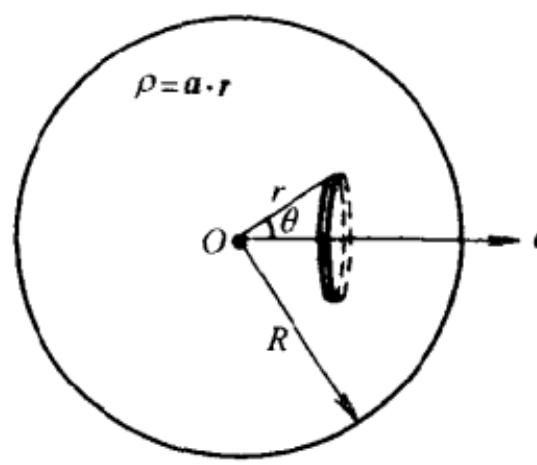
\includegraphics[width=0.5\linewidth]{figures/fig_1_2_32.jpg}
\end{center}

\vfill

\newpage

\textbf{1.2.33.} 用长为 $l$ 的细丝线系一个质量为 $m$ 的小球, 作成单摆, 如图 1.2.33 (1). 令小球带电荷量 $q$ 后, 放在一个匀强电场 $\pmb{E}$ 中, $\pmb{E}$ 的方向在竖直方向. (1) 试分别求 $\pmb{E}$ 向下和向上时, 这单摆的周期; (2) 在什么情况下周期比不带电时长?

\vfill

\textbf{1.2.34.} 一根均匀的刚体绝缘细杆, 质量为 $m$ , 用丝线拴住一端吊着, 并让它的两端分别带上电荷量 $q$ 和 $-q$ , 如图 1.2.34(1) 所示. 现在加上电场强度为 $E$ 的均匀电场, $E$ 沿水平方向. 试求静止时, 丝线与竖直方向的夹角 $\alpha$ ; 细杆与竖直方向的夹角 $\beta$ .

\vfill

\newpage

\textbf{1.2.35.} 把电偶极矩为 $p = ql$ 的电偶极子放在电荷量为 $Q$ 的点电荷的电场里， $p$ 的中心点 $O$ 到 $Q$ 的距离为 $r$ . 试分别求下列情况下它所受的力 $\pmb{F}$ 和力矩 $\pmb{M}: (1)p \parallel Q\vec{O}; (2)p \perp Q\vec{O}$ .

\vfill

\textbf{1.2.36.} 电偶极矩为 p 的电偶极子,处在电场强度为 E 的外电场中,p 与 E 的夹角为 $\theta$ ,如图 1.2.36 所示.(1)如果 E 是均匀电场, $\theta$ 为什么值时 p 达到平衡?是稳定平衡还是不稳定平衡?

图1.2.36

(2)如果 $\pmb{E}$ 不是均匀电场，试求 $\pmb{p}$ 所受的力的公式.
\begin{center}
    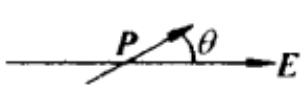
\includegraphics[width=0.5\linewidth]{figures/fig_1_2_36.jpg}
\end{center}

\vfill

\newpage

\textbf{1.2.37.} 电偶极矩为 $p$ 的电偶极子处在电场强度为 $\pmb{E}$ 的均匀外电场中，当 $p$ 平行于 $\pmb{E}$ 时达到平衡。如果让 $p$ 稍微偏离 $\pmb{E}$ 的方向，然后放手，则在 $\pmb{E}$ 的作用下，它便会作微小振动。已知它作这种振动的转动惯量为 $I$ ，试求振动频率。

\vfill

\textbf{1.2.38.} 在球坐标系中, 原点有一电荷量为 $Q$ 的点电荷, $P(r, \theta, \phi)$ 点有一电偶极子, 其电偶极矩为 $p = p(\cos \alpha e_r + \sin \alpha e_\theta)$ , 式中 $e_r$ 和 $e_\theta$ 分别是 $r$ 方向的单位矢量和 $\theta$ 方向 (即垂直于 $r$ 并指向 $\theta$ 增大的方向) 的单位矢量, 如图 1.2.38 所示. 试求 $Q$ 作用在这电偶极子上的力.

图1.2.38

图1.2.38(1)
\begin{center}
    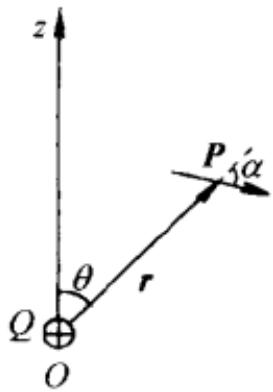
\includegraphics[width=0.5\linewidth]{figures/fig_1_2_38_1.jpg}
\end{center}
\begin{center}
    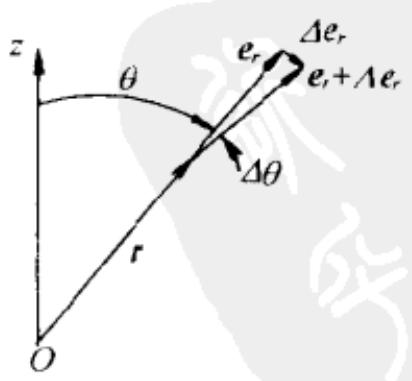
\includegraphics[width=0.5\linewidth]{figures/fig_1_2_38_2.jpg}
\end{center}

\vfill

\newpage

\textbf{1.2.39.} 如图 1.2.39(1) 所示, 电偶极矩分别为 $p_1$ 和 $p_2$ 的两个电偶极子, 在同一直线上, 方向相同, 相距为 $r$ . (1) 试证明: 它们之间相互作用力的大小为 $F = \frac{3p_1p_2}{2\pi\varepsilon_0r^4}$ , 力的方向是, $p_1$ 与 $p_2$ 同方向时互相吸引; 若 $p_1$ 与 $p_2$ 反方向, 则互相排斥. (2) 如果 $p_1$ 和 $p_2$ 是两个水分子的电偶极矩, 它们的值为 $p_1 = p_2 = 6.2 \times 10^{-30} \mathrm{C} \cdot \mathrm{m}$ , 它们间的距离为 $10 \mathrm{~nm}$ , 试计算它们间相互作用力的值.

图1.2.39(1)

图1.2.39(2)
\begin{center}
    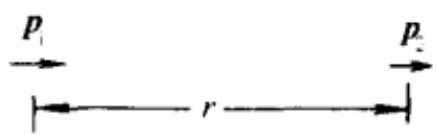
\includegraphics[width=0.5\linewidth]{figures/fig_1_2_39_1.jpg}
\end{center}
\begin{center}
    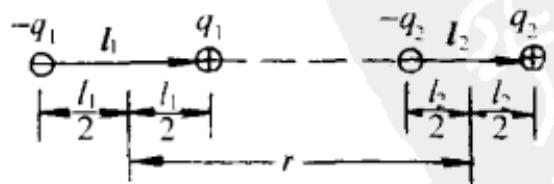
\includegraphics[width=0.5\linewidth]{figures/fig_1_2_39_2.jpg}
\end{center}

\vfill

\textbf{1.2.40.} 带电粒子在均匀外电场中运动时,它的轨迹是抛物线;试问这抛物线在什么情况下化为直线?

\vfill

\newpage

\textbf{1.2.41.} 质量为 $m$ 、电荷量为 $q$ 的粒子在电场强度为 $\pmb{E}$ 的均匀电场中运动，开始 $(t = 0)$ 时位矢为 $\pmb{r}_0$ ，速度为 $\pmb{v}_0$ ，试证明， $t$ 时刻它的位矢为 $\pmb{r} = \frac{q}{2m} Et^2 +\pmb{v}_0t + \pmb{r}_0.$

\vfill

\textbf{1.2.42.} 静质量为 m、电荷量为 q 的粒子在电场强度为 E 的均匀电场中由静止开始运动, 考虑狭义相对论, 其运动方程为

$$
\frac {\mathrm{d}}{\mathrm{d} t} \left(\frac {m \boldsymbol {v}}{\sqrt {1 - \frac {v ^ {2}}{c ^ {2}}}}\right) = q \boldsymbol {E}
$$

式中 $\pmb{v}$ 是粒子的速度， $c$ 是真空中光速。设以出发点为原点，沿 $\pmb{E}$ 的方向取 $x$ 轴，则 $v = \frac{\mathrm{d}x}{\mathrm{d}t}$ 。(1)试求粒子的坐标 $x$ 与时间 $t$ 的关系；(2)试证明，当 $t \to \infty$ 时，粒子的速度趋于 $c$ ；(3)试验证，当 $\frac{qE}{mc} t \ll 1$ 时，所得结果趋于非相对论的情况。

\vfill

\newpage

\textbf{1.2.43.} 一示波管用电场使电子偏转,如图 1.2.43 所示,偏转电极长为 l=电场使电子偏转,如图 1.2.43 所示,偏转电极长为 $l = 1.5 \mathrm{~cm}$ ,两极间是均匀电场,电场强度 $\pmb{E}$ 的大小为 $E = 1.2 \times 10^{4} \mathrm{~V} / \mathrm{m}$ .一电子以初速度 $\pmb{v}_{0}$ 进入这个电场, $\pmb{v}_{0}$ 与 $\pmb{E}$ 垂直.已知电子质量为 $m = 9.1 \times 10^{-31} \mathrm{~kg}$ ,电荷量的大小为 $e = 1.6 \times 10^{-19} \mathrm{C}$ ,初速度为 $\pmb{v}_{0} = 2.6 \times 10^{7} \mathrm{~m} / \mathrm{s}$ ,试求电子经过电极所发生的偏转 $y$ .

图1.2.43
\begin{center}
    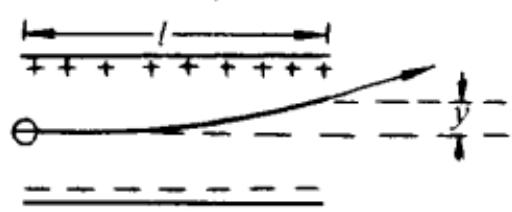
\includegraphics[width=0.5\linewidth]{figures/fig_1_2_43.jpg}
\end{center}

\vfill

\textbf{1.2.44.} 一电子以 $v_0 = 5.0 \times 10^7 \mathrm{~m/s}$ 的初速度射入电场强度为 $E$ 的均匀电场中, $E = 2.5 \times 10^5 \mathrm{~V/m}$ . 因 $v_0$ 与 $E$ 的方向相同, 电子因受电场力而减速. 已知电子的质量为 $m = 9.1 \times 10^{-31} \mathrm{~kg}$ , 电荷量的大小为 $e = 1.6 \times 10^{-19} \mathrm{C}$ , 试问这电子能穿入电场多少距离? 以后它会怎样? 它处在电场中的时间有多长?

\vfill

\newpage

\textbf{1.2.45.} 竖直放置的两块平行金属板 A、B 间有均匀电场，电场强度 E 的方向与板面垂直并由 A 指向 B，已知板长为 l [图 1.2.45(1)]. 有一正离子以初速度 $v_{0}$ 沿 A 板边缘竖直向下飞入电场中. 试问这离子在电场中运动多长时间，突然使电场反向（即 E 突然变为 -E），就能使它恰好从 A 板的下边缘飞出？重力比电场力小很多，可以略去不计.

图1.2.45(1)

图1.2.45(2)
\begin{center}
    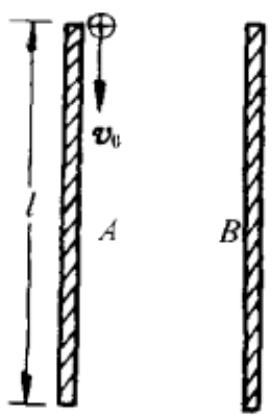
\includegraphics[width=0.5\linewidth]{figures/fig_1_2_45_1.jpg}
\end{center}
\begin{center}
    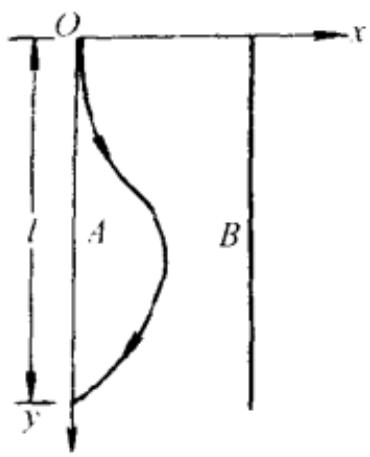
\includegraphics[width=0.5\linewidth]{figures/fig_1_2_45_2.jpg}
\end{center}

\vfill

\textbf{1.2.46.} 电场线是带单位正电荷量的粒子运动的轨迹吗？带电粒子会沿电场线运动吗？为什么？

\vfill

\newpage

\textbf{1.2.47.} 两个相同的点电荷,在它们联线的中点,电场线是否相交?为什么?

\vfill

\textbf{1.2.48.} 两个等量异号的点电荷, 相距为 $l$ , 以它们联线的中点为原点, 联线为 $x$ 轴, 取笛卡儿坐标系, 如图 1.2.48 所示. 试证明: 在 $xy$ 平面内, 它们的过 $(0, a)$ 点的电力线方程为

$$
\frac {x + l / 2}{\sqrt {(x + l / 2) ^ {2} + y ^ {2}}} - \frac {x - l / 2}{\sqrt {(x - l / 2) ^ {2} + y ^ {2}}} = \frac {2 l}{\sqrt {l ^ {2} + 4 a ^ {2}}}.
$$

图1.2.48
\begin{center}
    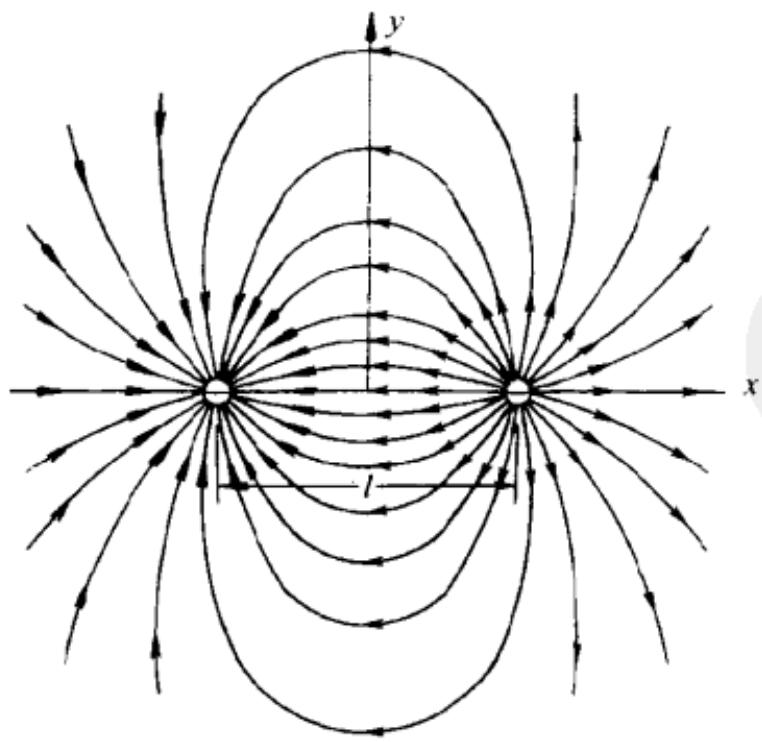
\includegraphics[width=0.5\linewidth]{figures/fig_1_2_48.jpg}
\end{center}

\vfill

\newpage

\textbf{1.2.49.} 两个等量同号的点电荷,相距为 l,以它们联线的中点为原点,联线为 x 轴,取笛卡儿坐标系,如图 1.2.49(1) 所示.试证明:在 xy 平面内,它们的电场线的方程为

$$
\frac {x + l / 2}{\sqrt {(x + l / 2) ^ {2} + y ^ {2}}} + \frac {x - l / 2}{\sqrt {(x - l / 2) ^ {2} + y ^ {2}}} = C
$$

式中 C 为常数.

\vfill

\textbf{1.3.1.} 高斯定理的表达式为 $\oiint_{S} \mathbf{E} \cdot \mathrm{d}\mathbf{S} = \frac{1}{\varepsilon_0} Q$ 。为什么此式左边的 $E$ 是高斯面 $S$ 内外所有电荷产生的电场强度，而右边的 $Q$ 却只是 $S$ 内的电荷而不包括 $S$ 外的电荷呢？

\vfill

\newpage

\textbf{1.3.2.} 有人认为:(1)如果高斯面上处处 E 为零,则该面内必无电荷;(2)如果高斯面内无电荷,则高斯面上处处 E 为零;(3)如果高斯面上处处 E 不为零,则高斯面内必有电荷;(4)如果高斯面内有电荷,则高斯面上处处 E 不为零.你认为以上这些说法是否正确？试分别举例说明.

\vfill

\textbf{1.3.3.} 电荷 $Q$ 均匀分布在一个球面上, 在球心有一电荷量为 $q$ 的点电荷. 由对称性和高斯定理可知: 球面上的电荷 $Q$ 在球心产生的电场强度为零, 因此, $Q$ 作用在 $q$ 上的力为零. 但 $q$ 在球面上产生的电场强度不为零, 因而 $q$ 有力作用在 $Q$ 上. 你认为这有矛盾吗?

\vfill

\newpage

\textbf{1.3.4.} 为了使电场线不仅表示电场强度 E 的方向,而且也表示 E 的大小,有人对电场线作如下规定:在电场中任一点,通过垂直于电场强度 E 的单位面积的电场线数目,等于该点 E 的量值.根据这个规定,一个质子发出多少条电场线?

\vfill

\textbf{1.3.5.} 电荷 $Q_{1}$ 均匀分布在半径为 $R_{1}$ 的球面上，电荷 $Q_{2}$ 均匀分布在半径为 $R_{2}$ 的同心球面上，如图1.3.5所示.(1)试求离球心为 $r$ 处的电场强度 $\pmb{E}$ ;(2)当 $Q_{2} = -Q_{1}$ 时各处的 $\pmb{E}$ 如何？

\vfill

\newpage

\textbf{1.3.6.} 半径分别为 $R_{1}$ 和 $R_{2}$ 的两个同心球面都均匀带电, 已知大球面上电为 $R_{1}$ 和 $R_{2}$ 的两个同心球面都均匀带电，已知大球面上电荷量的面密度为 $\sigma$ （图 1.3.6），大球面以外的电场强度为零。
(1)试求小球面上电荷量的面密度；(2)两球面间离球心为 r 处的电场强度 E；(3)小球面内的电场强度 $E_{i}$ .

图1.3.6
\begin{center}
    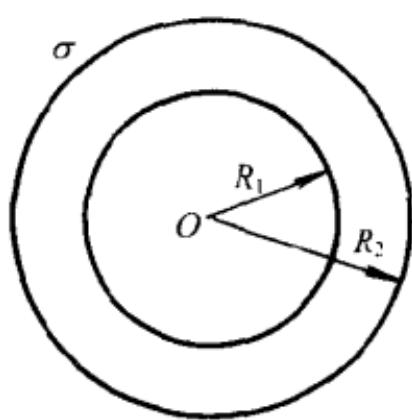
\includegraphics[width=0.5\linewidth]{figures/fig_1_3_6.jpg}
\end{center}

\vfill

\textbf{1.3.7.} 一球壳体的内外半径分别为 a 和 b，壳体中均匀分布着电荷，电荷量密度为 $\rho$ （图 1.3.7）。试求离球心为 r 处的电场强度 E，并画出 E-r 曲线（以 r 为横坐标，E 的大小 E 为纵坐标的 E 与 r 的关系曲线）。

\vfill

\newpage

\textbf{1.3.8.} 电荷 q 均匀地分布在半径为 R 的球体内, 试求离球心为 r 处的电场强度 E, 并画出 E 的大小 E 与 r 的关系曲线.

\vfill

\textbf{1.3.9.} 当电荷是球对称分布时,在这电荷外面任一点的电场强度,等于把这电荷都集中到球心时所产生的电场强度.试证明上述论断.在这电荷内部,上述论断是否适用?如果电荷不是球对称分布,上述论断是否适用?

\vfill

\newpage

\textbf{1.3.10.} 试论证:两个球对称分布的电荷系统之间的相互作用力等于它们的电荷都分别集中在各自球心成为两个点电荷之间的相互作用力.

图1.3.10(1)

【论证】一、具体说明 设电荷 $q_{1}$ 球对称地分布在半径为 $R_{1}$ 的球体内，电荷 $q_{2}$ 球对称地分布在半径为 $R_{2}$ 的球体内，两球心 $O_{1}$ 和 $O_{2}$ 相距为 $l (> R_{1} + R_{2})$ ，如图1.3.10(1)所示.因电荷量密度 $\rho_1(r)$ 和 $\rho_2(r)$ 都只是各自到中心 $O_{1}$ 和 $O_{2}$ 的距离 $r$ 的函数，故

$$
q _ {1} = 4 \pi \int_ {0} ^ {R _ {1}} \rho_ {1} (r) r ^ {2} \mathrm{d} r\tag{1}
$$

$$
q _ {2} = 4 \pi \int_ {0} ^ {R _ {2}} \rho_ {2} (r) r ^ {2} \mathrm{d} r\tag{2}
$$

## 二、论证步骤

要求论证: 这两个电荷系统之间的相互作用力等于 $q_{1}$ 集中在 $O_{1}, q_{2}$ 集中在 $O_{2}$ 所成的两个点电荷之间的相互作用力.

(1) 点电荷与球对称分布电荷之间的相互作用力. 考虑一电荷量为 $q_{1}$ 的点电荷和一电荷量为 $q_{2}$ 的球对称分布的电荷, 如图 1.3.10(2) 所示. 由于 $q_{2}$ 是球对称分布, 故由对称性和高斯定理可知, 它在 $q_{1}$ 点产生的电场强度等于 $q_{2}$ 集中在球心 $O_{2}$ 产生的电场强度. 由此得出:

图1.3.10(2)

结论一: 球对称分布的电荷 $q_{2}$ 对点电荷 $q_{1}$ 的作用力等于相应的点电荷 $q_{2}$ (即 $q_{2}$ 集中在球心 $O_{2}$ 所成的点电荷) 对点电荷 $q_{1}$ 的作用力.

因静止电荷之间的相互作用力遵守牛顿第三定律,故得出:

结论二: 点电荷 $q_{1}$ 对球对称分布的电荷 $q_{2}$ 的作用力等于点电荷 $q_{1}$ 对相应的点电荷 $q_{2}$ (即 $q_{2}$ 集中在球心 $O_{2}$ 所成的点电荷) 的作用力.

(2)球对称分布电荷 $q_{1}$ 与球对称分布电荷 $q_{2}$ 之间的相互作用力.如图1.3.10(1)，根据对称性和高斯定理，球对称分布电荷 $q_{1}$ 在球对称分布电荷 $q_{2}$ 所在处产生的电场强度，等于 $q_{1}$ 集中在球心 $O_{1}$ 产生的电场强度.由此得出：

结论三: 球对称分布电荷 $q_{1}$ 对球对称分布电荷 $q_{2}$ 的作用力等于相应的点电荷 $q_{1}$ (即电荷 $q_{1}$ 集中在球心 $O_{1}$ 所成的点电荷) 对球对称分布电荷 $q_{2}$ 的作用力.

又根据结论二，点电荷 $q_{1}$ 对球对称分布电荷 $q_{2}$ 的作用力，等于点电荷 $q_{1}$ 对相应的点电荷 $q_{2}$ （即电荷 $q_{2}$ 集中到球心 $O_{2}$ 所成的点电荷)的作用力.因此，球对称分布电荷 $q_{1}$ 对球对称分布电荷 $q_{2}$ 的作用力，便等于点电荷 $q_{1}$ 对相应的点电荷 $q_{2}$ 的作用力.于是我们得出：

结论四: 球对称分布电荷 $q_{1}$ 与球对称分布电荷 $q_{2}$ 之间的相互作用力, 等于相应的点电荷 $q_{1}$ (即电荷 $q_{1}$ 集中在 $O_{1}$ 所成的点电荷) 与相应的点电荷 $q_{2}$ (即电荷 $q_{2}$ 集中在 $O_{2}$ 所成的点电荷) 之间的相互作用力.
\begin{center}
    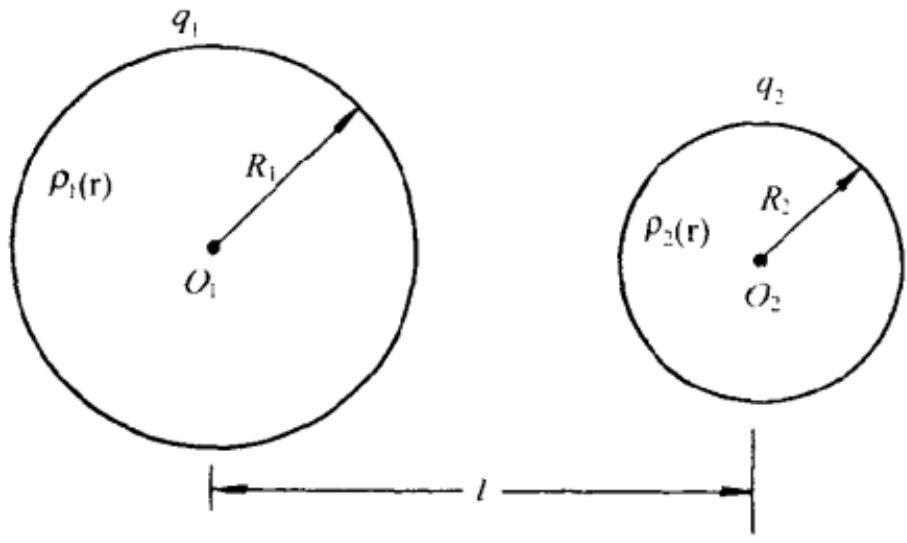
\includegraphics[width=0.5\linewidth]{figures/fig_1_3_10_1.jpg}
\end{center}
\begin{center}
    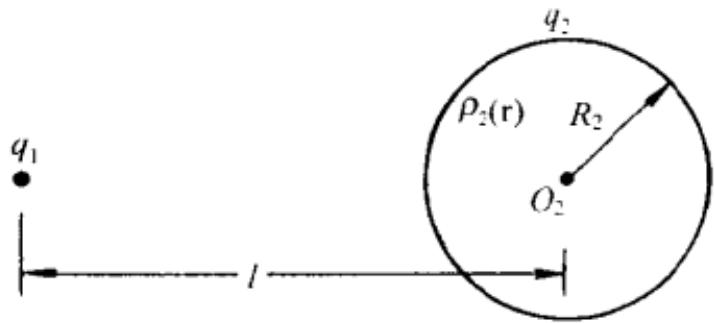
\includegraphics[width=0.5\linewidth]{figures/fig_1_3_10_2.jpg}
\end{center}

\vfill

\textbf{1.3.11.} 电荷均匀分布在一球体内,电荷量密度为 $\rho$ . (1)试求球内离球心为 $r$ 处的电场强度; (2)若在这球内挖去一部分电荷,挖去的体积是一个小球体,试求挖去电荷后空腔内的电场强度.

\vfill

\newpage

\textbf{1.3.12.} 空间有两个球, 球心间的距离小于它们的半径之和, 因此两球有一部分重叠, 如图 1.3.12 所示. 现在让两个球都充满均匀电荷, 电荷密度分别为 $\rho$ 和

图1.3.12

\- $\rho$ . 重叠部分由于正负电荷互相中和而无电荷. 试求重叠区域内的电场强度.
\begin{center}
    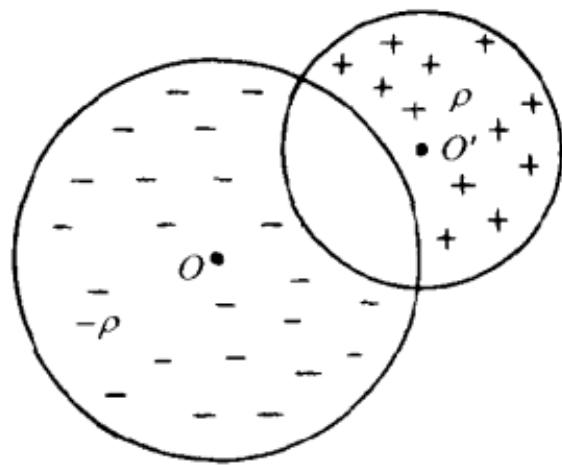
\includegraphics[width=0.5\linewidth]{figures/fig_1_3_12.jpg}
\end{center}

\vfill

\textbf{1.3.13.} 在半径为 R 的球体内, 挖一个半径为 $\frac{R}{2}$ 的球形空腔, 空腔的直径一端在球心 O, 另一端在球面上 A 点, 如图 1.3.13 所示, 把电荷量 q 均匀分布在未挖去的部分. 试求 OA 延长线上距球心为 r 处的 P 点的电场强度.

\vfill

\newpage

\textbf{1.3.14.} 在内外半径分别为 $a$ 和 $b$ 的球壳体内分布着电荷, 电荷量密度为 $\rho = \frac{A}{r}$ , 式中 $A$ 是常数, $r$ 是壳体内某一点到球心的距离. 现在球心放一电荷量为 $Q$ 的点电荷, 如图 1.3.14 所示. 要使壳体内各处电场强度的大小都相等, 试求 $A$ 的

值.

\vfill

\textbf{1.3.15.} 电荷分布在半径为 $R$ 的球体内，电荷量密度为 $\rho = \rho_0\left(1 - \frac{r}{R}\right)$ ，式中 $\rho_0$ 为常数， $r$ 为球心到球内一点的距离。试求：(1) 球内外离球心为 $r$ 处的电场强度；(2) 电场强度的最大值。

\vfill

\newpage

\textbf{1.3.16.} 根据量子力学, 氢原子处在基态时, 核外电荷的分布为 $\rho(r) = -\frac{q}{\pi a^3} \cdot e^{-\frac{2r}{a}}$ , 式中 $q = 1.60 \times 10^{-19} \mathrm{C}, a = 5.29 \times 10^{-11} \mathrm{~m}, r$ 是到原子核的距离. 试求: (1) 核外电荷的总电荷量; (2) 核外电荷在 $r$ 处产生的电场强度.

\vfill

\textbf{1.3.17.} 1903年,英国物理学家汤姆孙(J.J.Thomson)根据实验,提出“果子面包”型的原子模型:原子的正电荷均匀分布在半径约为 $1.0\times10^{-10}m$ 的球体内,原子的负电荷(即电子)则在正电荷球内运动.1911年,汤姆孙的学生卢瑟福(E.Rutherford)根据金核对α粒子的散射实验,提出原子的核模型:原子的正电荷集中在很小(约 $10^{-15}m$ )的范围内,电子则在核外运动.在原子范围内,这两种原子模型的正电荷所产生的电场强度是不相同的.以金原子为例,它的正电荷量为 $Ze=79\times1.6\times10^{-19}=1.26\times10^{-17}C$ ,它的原子核的半径为 $6.9\times10^{-15}m$ .(1)试求金原子核在它的表面上产生的电场强度的值;(2)按汤姆孙模型计算,金原子的正电荷所能产生的电场强度的值最大是多少?

\vfill

\newpage

\textbf{1.3.18.} 汤姆孙的氢原子模型是: 原子的正电荷量 e 均匀分布在半径为 R 的球体内, 原子的负电荷量 -e 集中成一个点电荷(即电子), 在正电荷的球体内运动. 设电子质量为 m, 某时刻的位矢为 r (从球心到电子的位置矢量). (1) 试求电子所受的力; (2) 若电子的初速度为零, 试证明它将作简谐振动, 并求振动频率; (3) 已知 $e = 1.6 \times 10^{-19}\mathrm{C}, m = 9.1 \times 10^{-31}\mathrm{kg}, R = 5.3 \times 10^{-11}\mathrm{m}$ , 计算频率的值.

\vfill

\textbf{1.3.19.} 一无穷长直线均匀带电,单位长度的电荷量为 $\lambda$ , 在它的电场的作用下,一质量为 m、电荷量为 q 的质点,以它为轴线作匀速圆周运动.试求质点的速率 v 和周期 T.

\vfill

\newpage

\textbf{1.3.20.} 两条平行的无穷长直线都均匀带电,单位长度的电荷量分别为 $\lambda$ 和 $-\lambda$ ,两线相距为 $a$ . (1) $P$ 为两线构成的平面内一点, $P$ 到中线(两带电线中间的平行线)的距离为 $r$ ,试求 $P$ 点的电场强度;(2)试求 $-\lambda$ 线单位长度所受的力.

\vfill

\textbf{1.3.21.} 半径为 $a$ 的无穷长直圆筒面均匀带电，沿轴线单位长度的电荷量为 $\eta$ 。试求离轴线为 $r$ 处的电场强度 $\pmb{E}$ ，并画出 $E - r$ 曲线（即以 $r$ 为横坐标，以 $\pmb{E}$ 的大小 $E$ 为纵坐标的 $E$ 与 $r$ 的关系曲线）。

\vfill

\newpage

\textbf{1.3.22.} 半径分别为 $R_{1}$ 和 $R_{2}(>R_{1})$ 的两无穷长直共轴圆筒，筒面上都均匀带电，沿轴线单位长度的电荷量分别为 $\lambda_{1}$ 和 $\lambda_{2}$ ，其中一段如图 1.3.22 所示。（1）试求(i)内筒内，(ii)两筒间和(iii)外筒外的电场强度；(2)当 $\lambda_{2} = -\lambda_{1}$ 时，各处的 E 如何？

\vfill

\textbf{1.3.23.} 半径为 R 的无限长直圆柱体内均匀地分布着电荷, 电荷量密度为

$\rho$ .试求离轴线为 $r$ 处的电场强度 $\pmb{E}$ ，并画出 $E - r$ 曲线.

图1.3.23
\begin{center}
    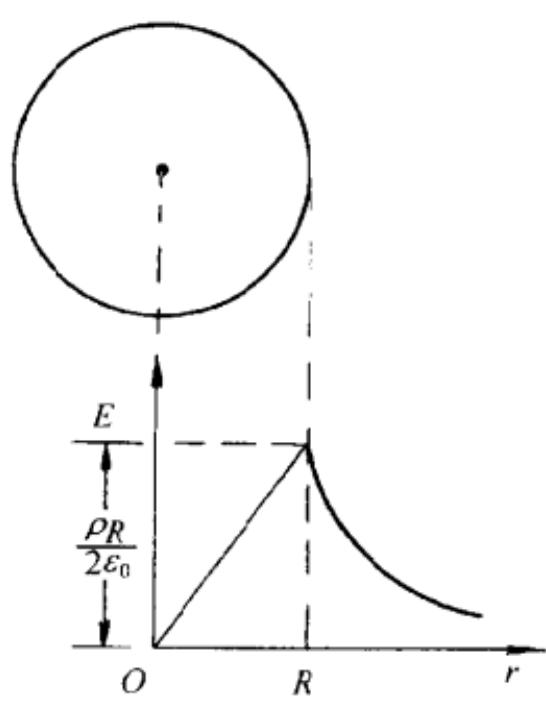
\includegraphics[width=0.5\linewidth]{figures/fig_1_3_23.jpg}
\end{center}

\vfill

\newpage

\textbf{1.3.24.} 电荷均匀分布在一无穷长圆柱体内,电荷量密度为 $\rho$ . 在这圆柱内挖出一无穷长圆柱形空腔,空腔的轴线与圆柱的轴线平行,相距为 $a$ ,横截面如图1.3.24所示.已知空腔内无电荷,试求空腔内的电场强度.

\vfill

\textbf{1.3.25.} 一无穷大平面均匀带电, 电荷量的面密度为 $\sigma$ , 离这平面为 $a$ 处, 有一质量为 $m$ 、电荷量为 $q$ 的粒子, 由于 $q\sigma < 0$ , 粒子受到带电平面的吸引. 设在开始 $(t = 0)$ 时, 粒子由静止因受平面电荷的吸引力而运动, 并且可以无阻碍地穿过电荷平面. 不考虑重力. 试求粒子的运动周期.

\vfill

\newpage

\textbf{1.3.26.} 两个无限大的平行平面都均匀带电,电荷量的面密度分别为 $\sigma$ 和 $-\sigma$ .试求各处的电场强度.

\vfill

\textbf{1.3.27.} 两个无限大的平行平面都均匀带电,电荷量的面密度相同,都是 $\sigma$ . 试求各处的电场强度.

\vfill

\newpage

\textbf{1.3.28.} 两个无限大的平行平面都均匀带电,电荷量的面密度分别为 $\sigma_{1}$ 和 $\sigma_{2}$ .试求各处的电场强度.

图1.3.28
\begin{center}
    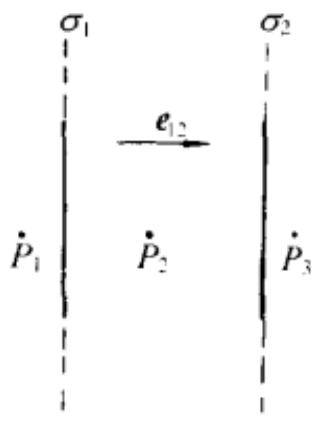
\includegraphics[width=0.5\linewidth]{figures/fig_1_3_28.jpg}
\end{center}

\vfill

\textbf{1.3.29.} 一厚度为 d 的无限大平板, 板内均匀地分布着电荷, 电荷量密度为 $\rho$ . 试求板内外离板中心为 r 处的电场强度.

\vfill

\newpage

\textbf{1.3.30.} 厚度都是 $a$ 的两块无限大平行平板, 板内都均匀地分布着电荷, 电荷量密度分别为 $\rho$ 和 $-\rho$ , 两板间距离为 $b$ , 如图 1.3.30(1) 所示. (1) 试求两板内外各处的电场强度 $E$ . (2) 如果两板有一部分重叠, 重叠部分的厚度为 $b$ , 如图 1.3.30(2) 所示, 结果如何?

\vfill

\textbf{1.3.31.} 实验表明,在靠近地面处有相当强的电场,电场强度 E 垂直于地面向下,大小约为 100V/m;在离地面 1.5km 高的地方,E 也是垂直于地面向下,大小约为 25V/m.试求地面附近大气中电荷量的平均密度.

\vfill

\newpage

\textbf{1.4.1.} 试用你自己的语言分别给(1)重力势能,(2)弹性势能(3)静电势能下定义.你能否从此得出一个统一的势能定义,使它对上述三种情况都适用?

\vfill

\textbf{1.4.2.} 在理论上,通常都把无穷远处的电势当作零;在实用上,通常都把地球的电势当作零.实验指出,如果把无穷远处的电势当作零,则地球的电势约为-8.2×10 $^{8}$ V.理论与实验不一致,你认为这矛盾如何解决?

\vfill

\newpage

\textbf{1.4.3.} 试回答下列问题:(1)电势高的地方电场强度是否大?电场强度大的地方电势是否高?(2)电场强度为零的地方,电势是否为零?电势为零的地方,电场强度是否为零?(3)电场强度大小相等的地方,电势是否相等?等势面上的电场强度是否相等?(4)电势为零的物体是否不带电?带正电的物体其电势是否是正的?

\vfill

\textbf{1.4.4.} 有人说：“在静电情况下，空间某一点的电势 $U$ 已定，该点电场强度 $\pmb{E}$ 的大小 $\pmb{E}$ 可以是任何值，方向可以是任何方向；反过来，该点的 $\pmb{E}$ 已定，该点的电势可以是任何值。因此，空间同一点的 $\pmb{E}$ 和 $U$ 没有直接关系。”你认为这种说法怎样？

\vfill

\newpage

\textbf{1.4.5.} 试证明下述论断: 在静电场中, 凡是电力线都是平行直线的地方, 电场强度的大小必定处处相等. 或者换句话说: 凡是电场强度的方向处处相同的地方, 电场强度的大小必定处处相等.

\vfill

\textbf{1.4.6.} 一个点电荷,电荷量为 q,在离它 10cm 处产生的电势为 100V,试求 q 的值.

\vfill

\newpage

\textbf{1.4.7.} 质子的电荷量为 $1.60 \times 10^{-19} \mathrm{C}$ , 质量为 $1.67 \times 10^{-27} \mathrm{~kg}$ , 金的原子核含有 79 个质子, 把它当做一个均匀带电的圆球, 半径为 $6.9 \times 10^{-15} \mathrm{~m}$ . 假定金原子核固定. (1) 一个质子以 $1.2 \times 10^{7} \mathrm{~m} / \mathrm{s}$ 的初速从很远处直射向金原子核, 试求它能达到金原子核的最近距离. (2) $\alpha$ 粒子的质量为 $6.7 \times 10^{-27} \mathrm{~kg}$ , 电荷量是质子的两倍, 它以 $1.6 \times 10^{7} \mathrm{~m} / \mathrm{s}$ 的初速从很远处直射向金原子核, 试求它能达到金原子核的最近距离.

\vfill

\textbf{1.4.8.} 一电子质量为 m，电荷量为 -e，以初速 $v_{0}$ 自很远处直射向一个固定的质子，质子的电荷量为 e。（1）试求电子的速度 v 与它们之间距离 r 的关系；（2）已知 $m = 9.11 \times 10^{-31} ~kg, e = 1.60 \times 10^{-19} ~C, v_{0} = 3.24 \times 10^{5} ~m/s$ ，试计算 $v = 2v_{0}$ 时 r 的值。

\vfill

\newpage

\textbf{1.4.9.} 已知电子的静质量为 $m_{0}=9.11\times10^{-31}kg$ ，电荷量为 $q=-1.60\times10^{-19}C$ 。(1) 设电子的质量不随速度变化，要把静止的电子加速到真空中光速 $c=2.9979\times10^{8}m/s$ ，试问它要经过多高的电压？(2) 对于高速运动的物体来说，上面的算法不对。因为根据狭义相对论，物体的质量 m 与它的速度 v 有关，关系为 $m=\frac{m_{0}}{\sqrt{1-v^{2}/c^{2}}}$ ，物体的动能不是 $\frac{1}{2}mv^{2}$ ，而是

$$
T = (m - m _ {0}) c ^ {2} = m _ {0} c ^ {2} \left(\frac {1}{\sqrt {1 - v ^ {2} / c ^ {2}}} - 1\right)
$$

按照这个公式,静止的电子经过上述电压加速后,速度是多少?是光速 c 的百分之几?(3)按照狭义相对论,要把带电粒子(静质量为 $m_{0}$ ,电荷量为 q)从静止加速到光速 c,需要经过多高的电压?

\vfill

\textbf{1.4.10.} 一电子二极管由半径为 $a = 5.0 \times 10^{-4} \mathrm{~m}$ 的圆柱形阴极 $K$ ，和套在 $K$ 外面的同轴圆筒形阳极 $A$ 构成， $A$ 的半径为 $b = 4.5 \times 10^{-3} \mathrm{~m}$ . $A$ 的电势比 $K$ 高 $300 \mathrm{~V}$ . 电子从 $K$ 出来时速度很小，可略去不计. 已知电子质量为 $9.1 \times 10^{-31} \mathrm{~kg}$ ，电荷量为 $-1.6 \times 10^{-19} \mathrm{C}$ . 试求：(1) 电子从 $K$ 向 $A$ 走过 $2.0 \mathrm{~mm}$ 时的速度值；(2) 电子到达 $A$ 时的速度值.

\vfill

\newpage

\textbf{1.4.11.} 一示波管如图 1.4.11 所示, 电子以 $v_{0}=2.4\times10^{7}m/s$ 的速度沿水平方向射入偏转电极间的均匀电场, 在这电场力的作用下向下偏转, 最后射到荧光屏上的 P 点. 已知偏转电极两金属板相距为 b=1.0cm, 长为 l=4.0cm, 偏转电极到荧光屏的距为 L=18cm; 偏转电极两板间电压为 160V; 电子质量为 $9.1\times10^{-31}kg$ , 电荷量为 -e=-1.6×

图1.4.11

$10^{-19}C$ .试求电子(1)在偏转电极间所受的力和产生的加速度;(2)射出偏转电极时速度在水平方向和竖直方向上的分量;(3)在荧光屏上的偏转距离.
\begin{center}
    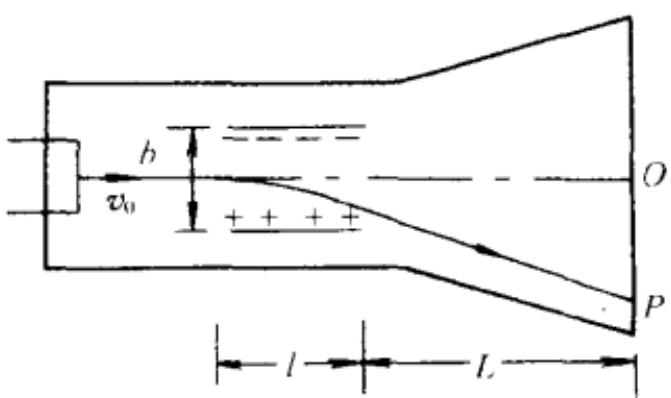
\includegraphics[width=0.5\linewidth]{figures/fig_1_4_11.jpg}
\end{center}

\vfill

\textbf{1.4.12.} 一示波管中电子以速度 $v_{0}$ 进入偏转极， $v_{0}$ 与偏转极中的电场强度

图1.4.12

垂直;已知电子质量为 m, 电荷量的大小为 e, 偏转极两板间的电压为 U, 两板相距为 d, 长都是 l, 板中心到荧光屏的距离为 L, 如图 1.4.12 所示. 试求电子的偏转距离 $y = y_{1} + y_{2}$ .
\begin{center}
    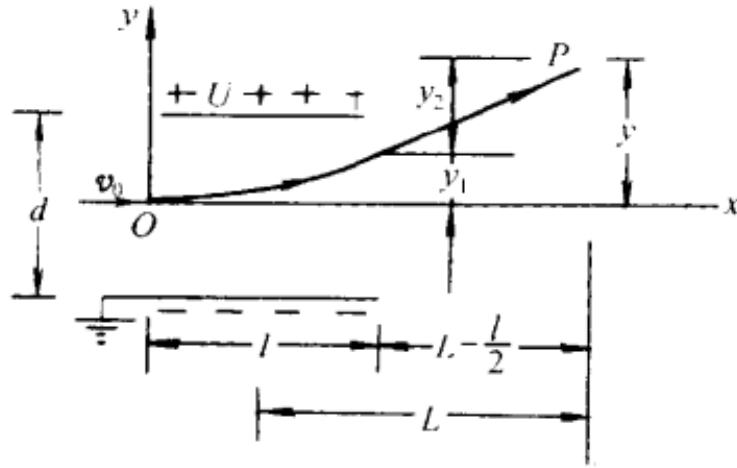
\includegraphics[width=0.5\linewidth]{figures/fig_1_4_12.jpg}
\end{center}

\vfill

\newpage

\textbf{1.4.13.} 半径为 $R$ 的光滑绝缘圆环, 固定在光滑绝缘的水平桌面上; 空间有水平方向的均匀电场, 电场强度为 $\pmb{E}$ , 如图1.4.13(1)所示, 图中纸面代表水平面. 在圆环内侧有一质量为 $m$ 、带有电荷量 $q$ 的质点, 它从 $P_{1}$ 位置以初速 $\pmb{v}_{0}(\pmb{v}_{0} \perp \pmb{E})$ 出发, 贴着圆环内侧作圆周运动. 为了使这质点经过图中 $P_{2}$ 位置 ( $P_{2}$ 与 $P_{1}$ 在同一直经的两端) 继续贴着圆环运动, 试求 $v_{0}$ 的取值范围.

\vfill

\textbf{1.4.14.} 一长为 $l$ 的丝线一端固定在 $O$ 点, 另一端系有质量为 $m$ 、电荷量为 $q (< 0)$ 的小球, 开始时, 丝线处于水平的伸直状态; 空间有电场强度为 $\pmb{E}$ 的均匀电场, $\pmb{E}$ 沿水平方向, 如图 1.4.14(1) 所示. 然后将小球自静止释放, 让它在重力和电场力的作用下摆动. 设丝线的质量和空气的阻力均可略去不计, $\pmb{E}$ 的大小为 $E = mg / |q|$ . (1) 试求 $m$ 第一次到达最低点所需的时间 $t$ ; (2) 设 $m$ 经过最低点后, 丝线一直处于伸直状态, 试求它达到左边水平位置时速度的大小 $v$ .

图1.4.13(2)

图1.4.14(1)

图1.4.14(2)
\begin{center}
    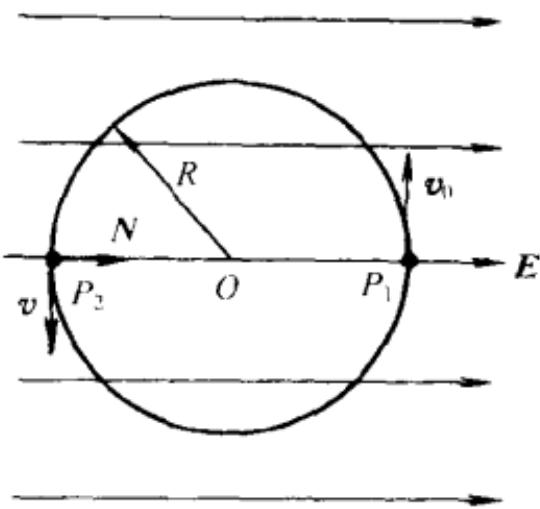
\includegraphics[width=0.5\linewidth]{figures/fig_1_4_14_1.jpg}
\end{center}
\begin{center}
    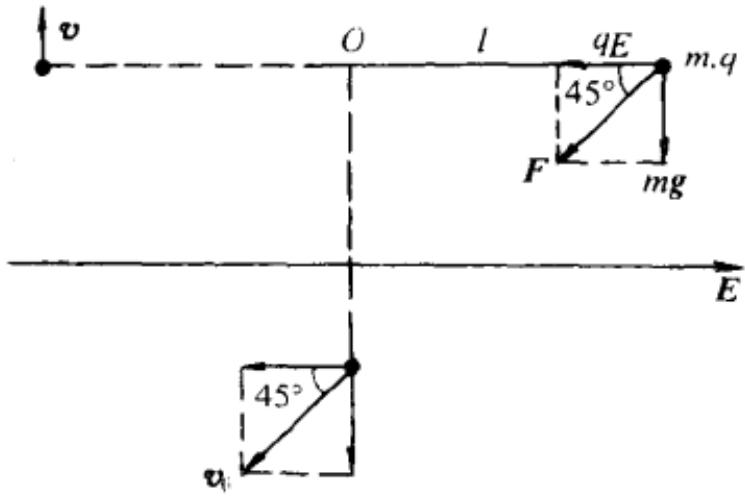
\includegraphics[width=0.5\linewidth]{figures/fig_1_4_14_2.jpg}
\end{center}
\begin{center}
    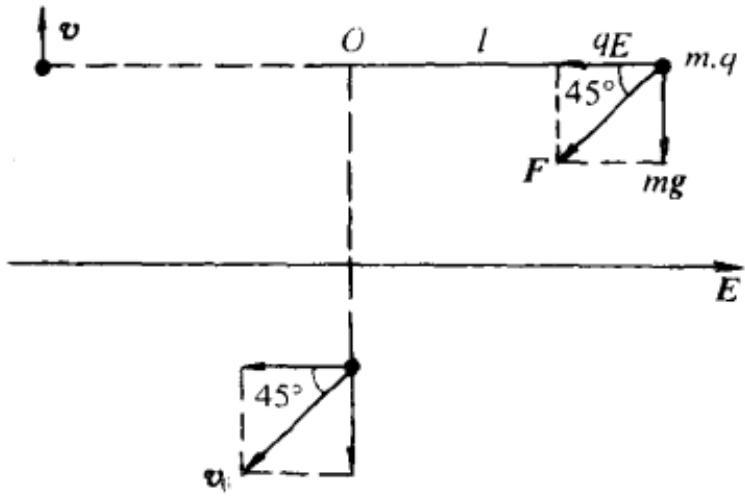
\includegraphics[width=0.5\linewidth]{figures/fig_1_4_14_3.jpg}
\end{center}

\vfill

\newpage

\textbf{1.4.15.} 氢原子由一个质子(即氢原子核)和一个电子组成,根据经典模型,氢原子在基态时,电子环绕质子作匀速圆周运动,轨道的半径为 $a = 5.29 \times 10^{-11} ~m$ . 已知电子和质子的电荷量的大小都是 $e = 1.60 \times 10^{-19} ~C$ . 把基态氢原子的电子和质子分开到相距无穷远所需的最小能量叫做氢原子的电离能量,试求这个能量的值. 1 mol 氢原子(即 $6.02 \times 10^{23}$ 个氢原子)的电离能量是多少?

\vfill

\textbf{1.4.16.} 实验表明,轻原子核结合成为较重的原子核时(称为核聚变),能放出大量的能量.例如,四个氢原子核(质子)结合成一个氦原子核( $\alpha$ 粒子)时,可放出28MeV的能量.这种核聚变就是太阳发光发热的能量来源.近五十年来,人们一直在研究如何在地球上实现受控的核聚变,以便解决人类的能源问题.实现核聚变的困难在于原子核都带正电,互相排斥,在一般情况下不能互相靠近而发生结合.只有在温度非常高时,原子核热运动的速度非常快,才能冲破斥力而碰到一起,发生结合(称为热核聚变).根据统计物理学,温度为T时,粒子的平均平动能为 $\frac{1}{2}m\overline{v^{2}}=\frac{3}{2}kT$ ,式中 $k=1.38\times10^{-23}J/K$ ,称为玻耳兹曼常量.已知质子的电荷量为 $e=1.60\times10^{-19}C$ ,半径约为 $r=1\times10^{-15}m$ .试计算两个质子因热运动而达到互相接触时所需的最低温度.

\vfill

\newpage

\textbf{1.4.17.} 当空气中的电场强度达到 $2 \times 10^{6} ~V/m$ 时, 空气便会被击穿而发生火花放电. 测得某次雷电的火花长 100 米, 试求这次闪电时两端的电势差.

\vfill

\textbf{1.4.18.} 在夏季雷雨时,通常一次闪电里两端的电势差约为十亿伏特,通过的电量约为30C.试问一次闪电消耗的能量是多少?如果这些能量用来烧水,试问能把多少水从0℃加热到100℃?

\vfill

\newpage

\textbf{1.4.19.} 一个电子经过1伏特的电势差时，它的电势能之差称为电子伏，以eV表示，是原子物理学中常用的能量单位；在原子核物理学中，能量较高，常用兆电子伏(MeV)作单位， $1MeV=10^{6}eV$ ；在高能物理学中，能量更高，常用吉电子伏(GeV)作单位， $1GeV=10^{9}eV$ 。已知电子电荷的大小为 $1.602\times10^{-19}C$ ，试分别求1eV、1MeV和1GeV各等于多少焦耳？一盏4W电灯点一小时，所用的电能等于多少eV？

$$
\begin{array}{r l} {\text {   【解   } ]} & {1 \mathrm{eV} = 1. 6 0 2 \times 1 0 ^ {- 1 9} \times 1 = 1. 6 0 2 \times 1 0 ^ {- 1 9} (\mathrm{J})} \\ & {1 \mathrm{MeV} = 1 0 ^ {6} \mathrm{eV} = 1. 6 0 2 \times 1 0 ^ {- 1 3} (\mathrm{J})} \\ & {1 \mathrm{GeV} = 1 0 ^ {9} \mathrm{eV} = 1. 6 0 2 \times 1 0 ^ {- 1 0} (\mathrm{J})} \end{array}
$$

40 瓦电灯一小时用的电能为

$$
W = \frac {4 0 \times 6 0 \times 6 0}{1 . 6 0 2 \times 1 0 ^ {- 1 9}} = 9. 0 \times 1 0 ^ {2 3} (\mathrm{eV})
$$

\vfill

\textbf{1.4.20.} 由统计物理学得出, 当热力学温度为 T 时, 微观粒子热运动能量的数量级为 kT, 其中 $k = 1.38 \times 10^{-23}$ J/K 是玻耳兹曼常量. 因此, 可以用能量表示温度. 当 kT 的值为多少 eV 时, 就说它的温度 T 等于多少 eV. 试问: (1) T = 1eV 时是多少 K? (2) T = 50keV 时是多少 K? (3) 室温 (T = 300K) 时 T 是多少 eV? (4) 太阳表面温度约 6000K, T 是多少 eV? (5) 热核反应时温度高达 $10^{8}$ K, T 是多少 eV?

\vfill

\newpage

\textbf{1.4.21.} 图 1.4.21 的 (1)、(2)、(3) 中两点电荷的电荷量都已标明是 $Q$ 或 $-Q$ , 它们相距都是 $l, P$ 都是联线的中点. 试分别求三种情况下 $P$ 点的电场强度 $E$ 和电势 $U$ .

\vfill

\textbf{1.4.22.} 在电荷量为 $Q$ 的点电荷所产生的电场中有 $A, B, C$ 三点， $A$ 点离 $Q$ 为 $r, B, C$ 两点离 $Q$ 均为 $2r$ ，如图1.4.22所示。现将电荷量为 $q$ 的点电荷从 $A$ 移到 $B$ ，试求电场力做的功 $W_{AB}$ ；将 $q$ 从 $A$ 移到 $C$ ，试求电场力做的功 $W_{AC}$ 。若将 $q$ 从 $B$ 移到 $C$ ，电场力做的功是多少？

图1.4.22
\begin{center}
    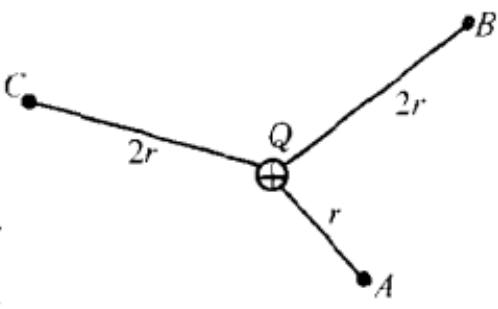
\includegraphics[width=0.5\linewidth]{figures/fig_1_4_22.jpg}
\end{center}

\vfill

\newpage

\textbf{1.4.23.} 图 1.4.23 中 A、O、B、D 在一直线上，其间距离如图所示，OCD 是

图1.4.23

半径为 $l$ 的半圆； $A$ 点和 $B$ 点分别有电荷量为 $q$ 和 $-q$ 的点电荷。试求：(1) 把单位正电荷量从 $O$ 点沿半圆弧 $\overline{OCD}$ 移到 $D$ 点，电场力做的功；(2) 把单位负电荷量从 $D$ 点沿 $AD$ 的延长线移到无穷远去，电场力做的功。
\begin{center}
    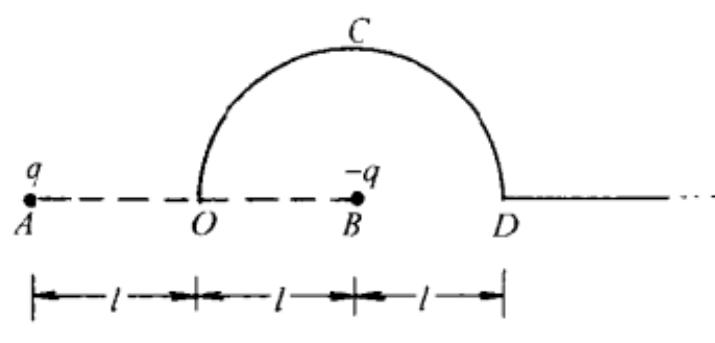
\includegraphics[width=0.5\linewidth]{figures/fig_1_4_23.jpg}
\end{center}

\vfill

\textbf{1.4.24.} 在边长为 $a$ 的正方形顶点, 各有一个固定的点电荷, 它们的电荷量分别为 $Q$ 、 $-Q$ 、 $Q$ 和 $-Q$ , 如图 1.4.24 所示. 现将电荷量为 $q$ 的点电荷从中心 $O$ 移到右边的中点 $P$ , 试求电场力对它做的功. 如果四个点电荷的电荷量都是 $Q$ , 则 $q$ 从 $O$ 移到 $P$ , 电场力对它做的功又是多少?
\begin{center}
    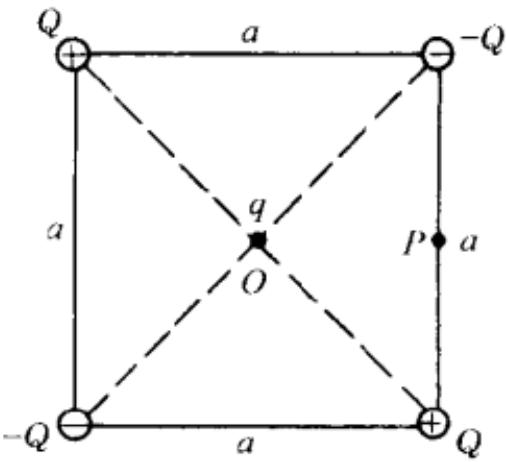
\includegraphics[width=0.5\linewidth]{figures/fig_1_4_24.jpg}
\end{center}

\vfill

\newpage

\textbf{1.4.25.} 电荷量分别为 $q$ 和 $-q$ 的两个点电荷, 相距为 $l$ , 以它们联线的中点 $O$ 为原点, 联线为极轴, 取极坐标系, 如图 1.4.25 所示, 试求 $q$ 和 $-q$ 在 $P(r, \theta)$ 点产生的电势. 当 $r \gg l$ 时, 结果如何?

图1.4.25

图1.4.25(1)
\begin{center}
    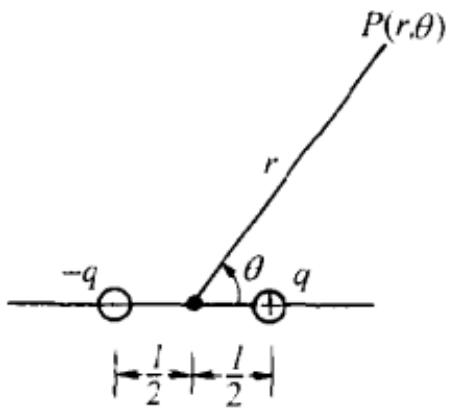
\includegraphics[width=0.5\linewidth]{figures/fig_1_4_25_1.jpg}
\end{center}
\begin{center}
    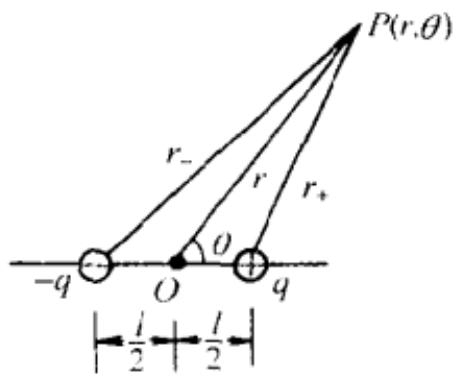
\includegraphics[width=0.5\linewidth]{figures/fig_1_4_25_2.jpg}
\end{center}

\vfill

\textbf{1.4.26.} 电荷量分别为 $q$ 和 $-q$ 的两个点电荷，相距为 $l$ ，以它们联线的中点

图1.4.26

O 为原点, 联线为 x 轴, 取笛卡儿坐标系, 如图 1.4.26 所示, 试求 q 和 -q 在 $P(x, y)$ 点产生的电势. 当 $\sqrt{x^{2} + y^{2}} \gg l$ 时, 结果如何?
\begin{center}
    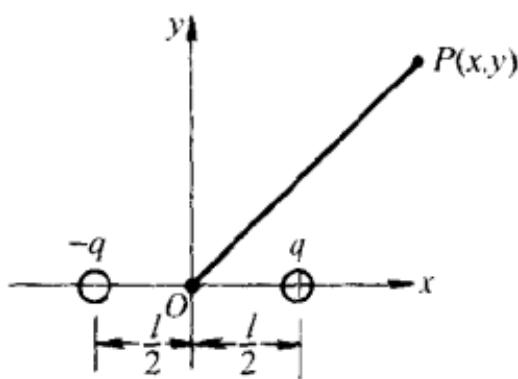
\includegraphics[width=0.5\linewidth]{figures/fig_1_4_26.jpg}
\end{center}

\vfill

\newpage

\textbf{1.4.27.} 电荷量分别为 $q$ 和 $-q$ 的两个点电荷, 相距为 $l$ ; 对于离它们很远 (即到它们的距离比 $l$ 大很多) 的区域来说, 这两个电荷构成的系统称为电偶极子, $p = ql$ 称为它的电偶极矩, 式中 $l$ 是从 $-q$ 到 $q$ 的位矢. 以电偶极子的中心 $O$ 为原点, $l$ 为极轴, 取极坐标系, 如图 1.4.27 所示. 试求它在 $P(r, \theta)$ 点产生的电势 $U$ , 并由 $U$ 求电场强度 $E$ .
\begin{center}
    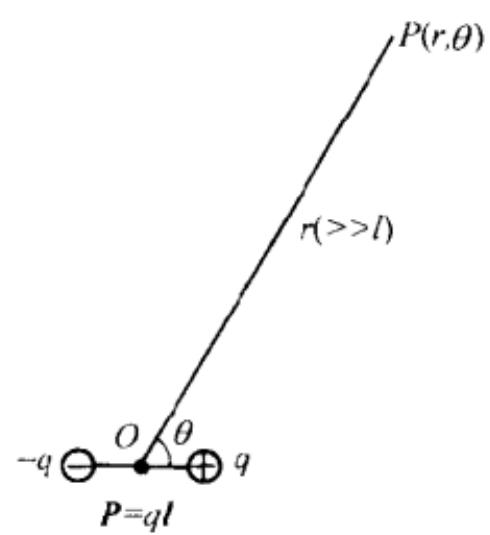
\includegraphics[width=0.5\linewidth]{figures/fig_1_4_27.jpg}
\end{center}

\vfill

\textbf{1.4.28.} 电荷量分别为 q 和 -q 的两个点电荷, 相距为 l, 以它们联线的中点 O 为原点, 联线为 x 轴, 取笛卡儿坐标系, 如图 1.4.28 所示. 试求这两个点电荷的等势面方程. 当它们可以当作电偶极子时, 结果如何?

\vfill

\newpage

\textbf{1.4.29.} 有两个异号的点电荷,电荷量分别为 $ne(n > 1)$ 和 $-e$ ,相距为 $a$ . 试证明:电势为零的等势面是一个球面,球心在它们间联线的延长线上 $-e$ 的外边.

\vfill

\textbf{1.4.30.} 如图 1.4.30, 在 x 轴上有两个点电荷, 电荷量为 q 的点电荷在 x = a 处, 电荷量为 $-\frac{R}{a}q$ 的点电荷在 $x = \frac{R^{2}}{a}$ 处. 试证明: 以原点 O 为心、R 为半径的球面是电势为零的等势面.
\begin{center}
    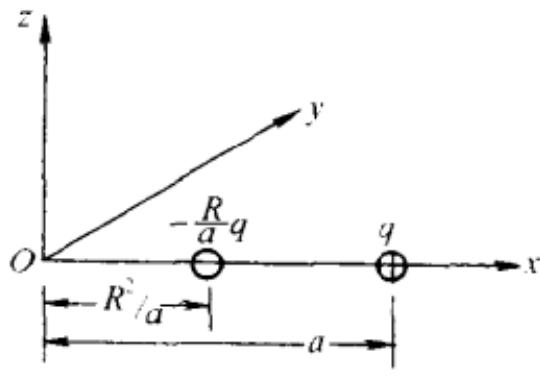
\includegraphics[width=0.5\linewidth]{figures/fig_1_4_30.jpg}
\end{center}

\vfill

\newpage

\textbf{1.4.31.} 电荷量分别为 $-\frac{a}{b} q, q, q$ 和 $-\frac{a}{b} q$ 的四个点电荷，对称地分布在 $x$ 轴上，它们的坐标分别为 $-\frac{a^2}{b}, -b, b$ 和 $\frac{a^2}{b}$ ，如图1.4.31所示 $(a, b > 0)$ 。试证明：以 $a$ 为半径的球面（球心在原点 $O$ ）是电势为零的等势面。

图1.4.31
\begin{center}
    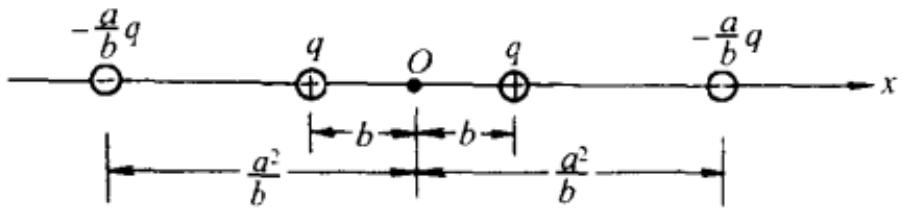
\includegraphics[width=0.5\linewidth]{figures/fig_1_4_31.jpg}
\end{center}

\vfill

\textbf{1.4.32.} 一电偶极矩为 p 的电偶极子处在外电场中, 它所在处的外电场强度

图1.4.32

为 E.(1)试求它的电势能 W;(2)在什么情况下 W 最小,其值是多少?(3)在什么情况下 W 最大,其值是多少?
\begin{center}
    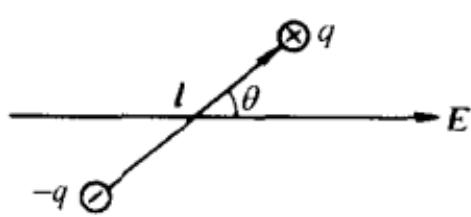
\includegraphics[width=0.5\linewidth]{figures/fig_1_4_32.jpg}
\end{center}

\vfill

\newpage

\textbf{1.4.33.} 电偶极矩为 p 的电偶极子处在电场强度为 E 的均匀外电场中, 试证明: 要将它的 p 翻转 $180^{\circ}$ , 外力须作功 $2p \cdot E$ .

\vfill

\textbf{1.4.34.} 四个点电荷在同一直线上, 电荷量为 $q$ 的两个点电荷相距为 $2l$ , 在它们的联线中点, 电荷量为 $-q$ 的两个点电荷重合在一起, 如图 1.4.34 所示. 对于 $r \gg l$ 处的 $P(r, \theta)$ 点来说, 这个电荷系统称为线性电四极子. 试证明: 这线性电四极子在 $P(r, \theta)$ 点产生的电势和电场强度分别为

$$
U = \frac {q l ^ {2}}{4 \pi \varepsilon_ {0} r ^ {3}} (3 \cos^ {2} \theta - 1)
$$

$$
\boldsymbol {E} = \frac {3 q l ^ {2}}{4 \pi \varepsilon_ {0} r ^ {4}} \left[ (3 \cos^ {2} \theta - 1) e _ {r} + 2 \sin \theta \cos \theta e _ {r} \right]
$$

图1.4.34
\begin{center}
    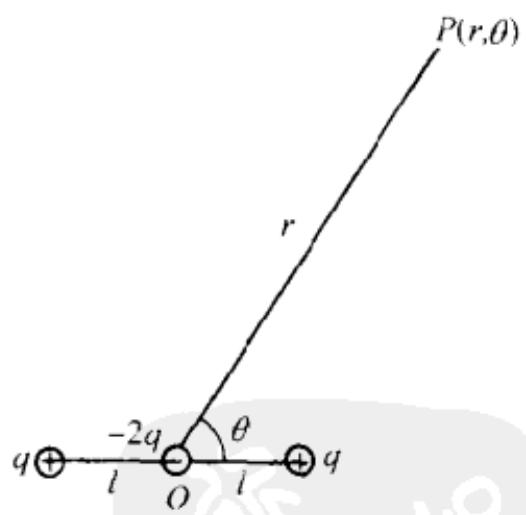
\includegraphics[width=0.5\linewidth]{figures/fig_1_4_34.jpg}
\end{center}

\vfill

\newpage

\textbf{1.4.35.} 四个点电荷分别处在边长为 $l$ 的正方形的四个顶点，电荷量分别为 $q$ 和 $-q$ ，如图1.4.35(1)所示.以正方形中心 $O$ 为原点，取极坐标系，使极轴平行于两边；空间一点 $P(r,\theta)$ 与电荷在同一平面内.对于 $r\gg l$ 的区域来说，这四个点电荷构成的电荷系统称为平面电四极子.(1)试证明：这个平面电四极子在 $P(r,$

$\theta)$ 点产生的电势为

$$
U = - \frac {3 q l ^ {2} \sin \theta \cos \theta}{4 \pi \varepsilon_ {0} r ^ {3}}
$$

图1.4.35(1)

图1.4.35(2)

(2)由 U 求该点的电场强度 E.
\begin{center}
    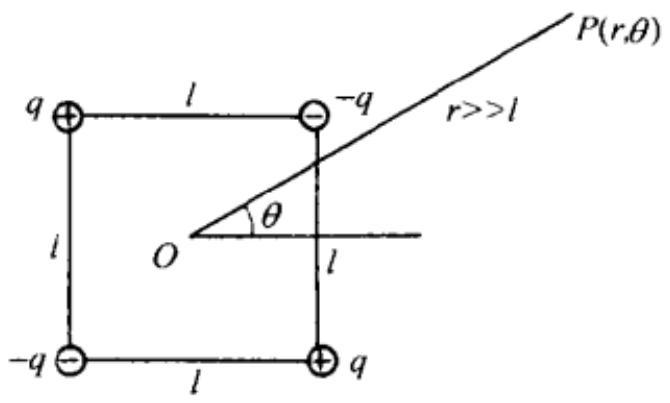
\includegraphics[width=0.5\linewidth]{figures/fig_1_4_35_1.jpg}
\end{center}
\begin{center}
    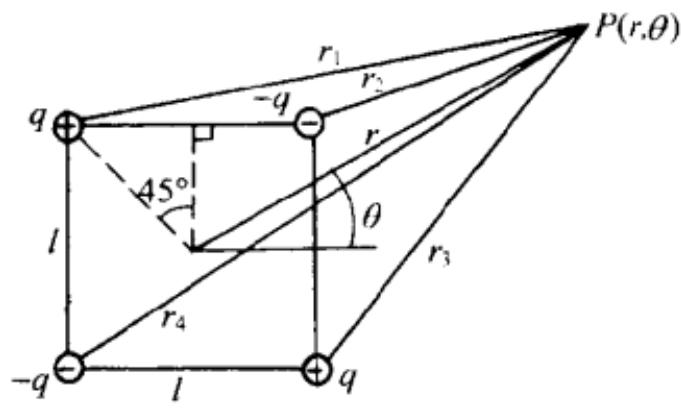
\includegraphics[width=0.5\linewidth]{figures/fig_1_4_35_2.jpg}
\end{center}

\vfill

\textbf{1.4.36.} 电荷量 q 均匀地分布在长为 2l 的一段直线上, 以这线段的中心 O 为原点取笛卡儿坐标系, 使这线段在 x 轴上, 如图 1.4.36(1) 所示. $P(x,y,z)$ 为这线段外的空间任一点, 试求 q 在 $P(x,y,z)$ 点产生的电势.

\vfill

\newpage

\textbf{1.4.37.} 电荷量 $q$ 均匀地分布在长为 $2l$ 的一段直线上, 如图 1.4.37(1) 和图 1.4.37(2) 所示, 试求下列各处的电势 $U$ , 并由 $U$ 求电场强度 $\pmb{E}$ : (1) 中垂面上离中心 $O$ 为 $r_1$ 处; (2) 延长线上离 $O$ 为 $r_2$ 处; (3) 端垂面 (通过一端并垂直于直线段的平面) 上离该端为 $r_3$ 处.

图1.4.37(1)

图1.4.37(2)
\begin{center}
    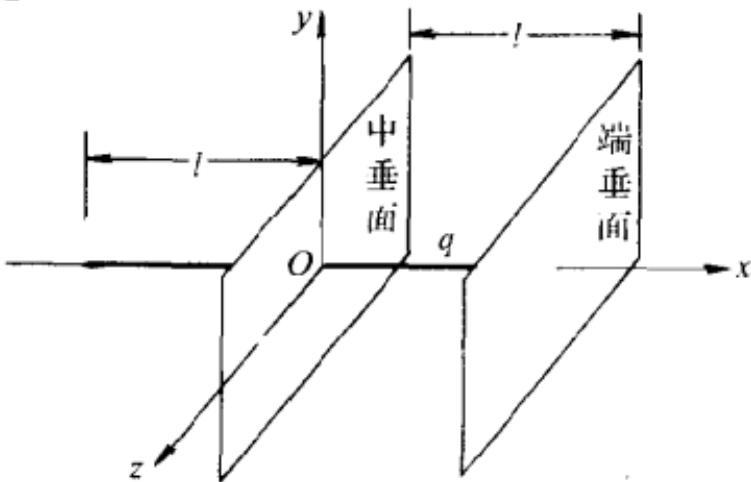
\includegraphics[width=0.5\linewidth]{figures/fig_1_4_37_1.jpg}
\end{center}
\begin{center}
    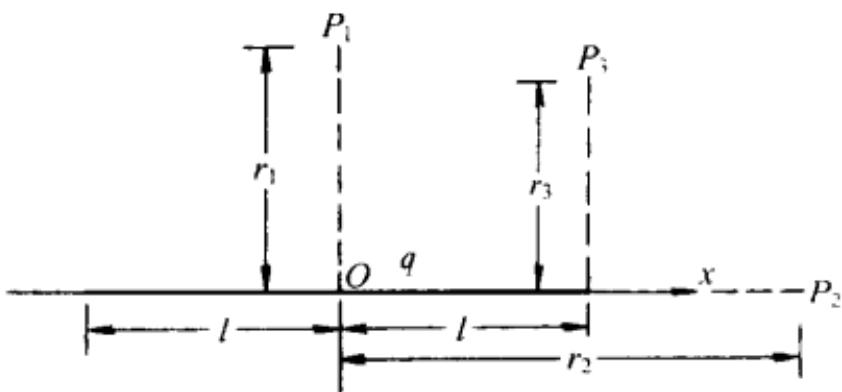
\includegraphics[width=0.5\linewidth]{figures/fig_1_4_37_2.jpg}
\end{center}

\vfill

\textbf{1.4.38.} 一段直线均匀带电,试证明:其等势面是以该直线两端为焦点、并以该直线为轴的旋转椭球面.

\vfill

\newpage

\textbf{1.4.39.} 一条无穷长直线均匀带电,单位长度的电荷量为 $\lambda$ .试求离这直线分

图1.4.39

别为 $r_{1}$ 和 $r_{2}$ 的两点的电势差.
\begin{center}
    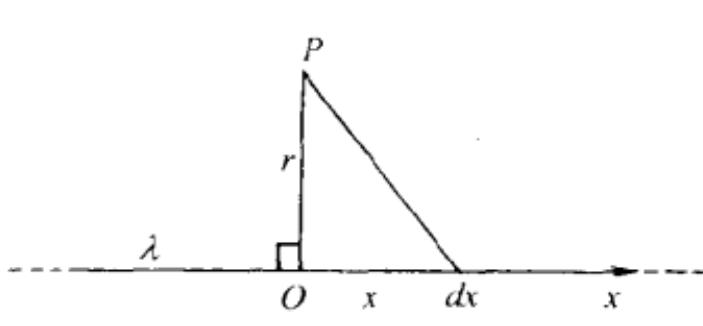
\includegraphics[width=0.5\linewidth]{figures/fig_1_4_39.jpg}
\end{center}

\vfill

\textbf{1.4.40.} 两条都均匀带电的无穷长平行直线,单位长度的电荷量分别为 $\lambda$ 和


\- $\lambda$ ，相距为 $2a$ ，如图1.4.40所示（图中两带电直线都与纸面垂直），试求空间任一点 $P(x,y)$ 的电势.
\begin{center}
    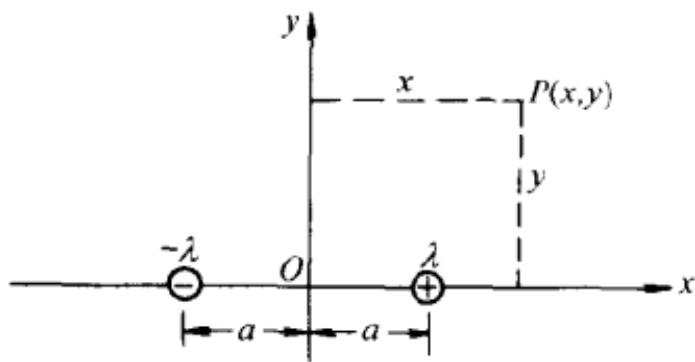
\includegraphics[width=0.5\linewidth]{figures/fig_1_4_40.jpg}
\end{center}

\vfill

\newpage

\textbf{1.4.41.} 两条均匀带电的无穷长平行直线, 相距为 $2a$ , 单位长度的电荷量分别为 $\lambda$ 和 $-\lambda$ ; 以两带电线构成的平面为 $z - x$ 平面, 使 $z$ 轴与两线平行且距离相等, 取笛卡儿坐标系如图 1.4.41(1) 所示. 试证明: (1) 电势为 $U$ 的等势面是半径为 $r = \left| \frac{2ka}{k^2 - 1} \right|$ 的圆柱面, 其中 $k = \mathrm{e}^{2\pi \varepsilon_0 U / \lambda}$ , 圆柱的轴线与两带电的直线平行且共面, 位置在 $x$ 轴上 $x_0 = \frac{k^2 + 1}{k^2 - 1} a$ 处; (2) 在 $x - y$ 平面内, 电场线的方程为 $x^2 + y^2 -$ $by - a^{2} = 0$ , 即圆心在 y 轴上的圆, 其中 b 为常数.

图1.4.41(1)
\begin{center}
    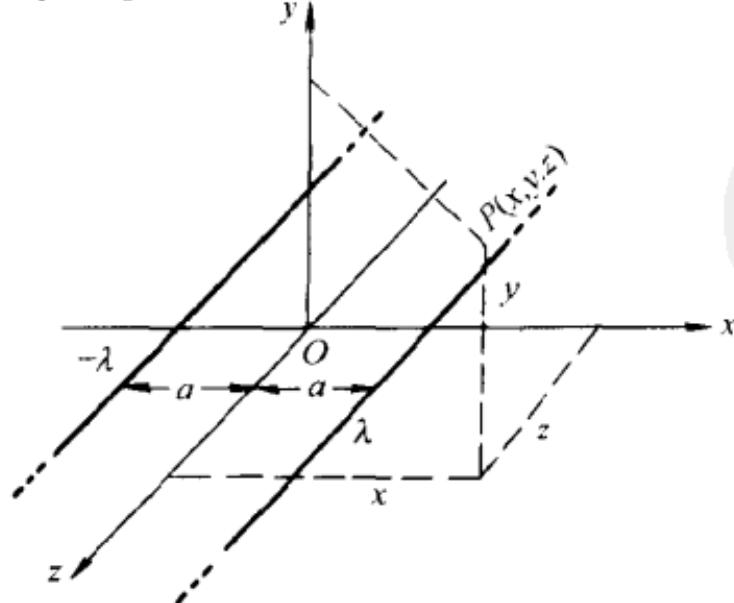
\includegraphics[width=0.5\linewidth]{figures/fig_1_4_41.jpg}
\end{center}

\vfill

\textbf{1.4.42.} 电荷量 q 均匀分布在长为 4l 的一段直线上，在电荷分布不变的情况下，把这段直线弯成边长为 l 的正方形。(1)试求这正方形轴线上离中心为 r 处的电势；(2)试证明：在 $r \gg l$ 处，这电势相当于点电荷 q 产生的电势。
\begin{center}
    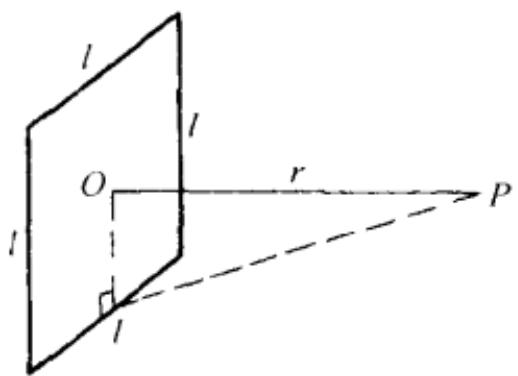
\includegraphics[width=0.5\linewidth]{figures/fig_1_4_42.jpg}
\end{center}

\vfill

\newpage

\textbf{1.4.43.} 电荷量 q 均匀地分布在半径为 R 的圆环上, P 为圆环轴线上离环心

图1.4.43(1)

为 $r$ 的一点, 如图1.4.43(1)所示. (1)试求 $P$ 点的电势 $U$ , 并由 $U$ 求电场强度 $\pmb{E}$ ; (2)试求 $P$ 点的电场强度 $\pmb{E}$ , 并由 $\pmb{E}$ 求电势 $U$ ; (3)以 $r$ 为横坐标, $U$ 为纵坐标, 画出 $U - r$ 曲线.
\begin{center}
    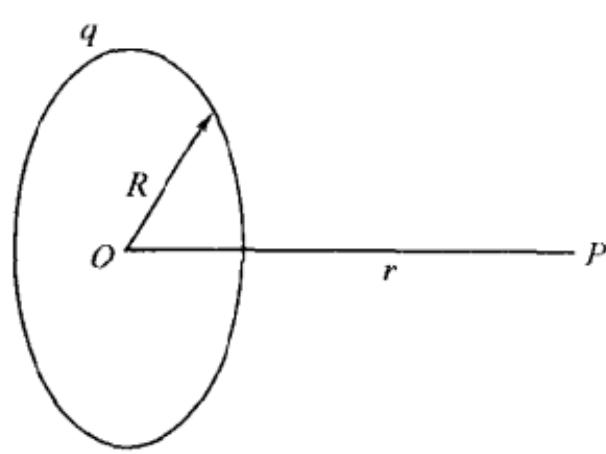
\includegraphics[width=0.5\linewidth]{figures/fig_1_4_43.jpg}
\end{center}

\vfill

\textbf{1.4.44.} 电荷量 q 均匀分布在半径为 R 的圆环上, 如图 1.4.44(1) 所示. 试证明: 轴线外任一点 $P(r, \theta)$ 的电势 U 的准确表达式是一个椭圆积分.

图1.4.44(1)

图1.4.44(2)
\begin{center}
    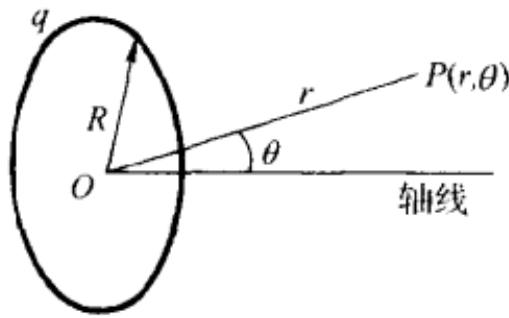
\includegraphics[width=0.5\linewidth]{figures/fig_1_4_44_1.jpg}
\end{center}
\begin{center}
    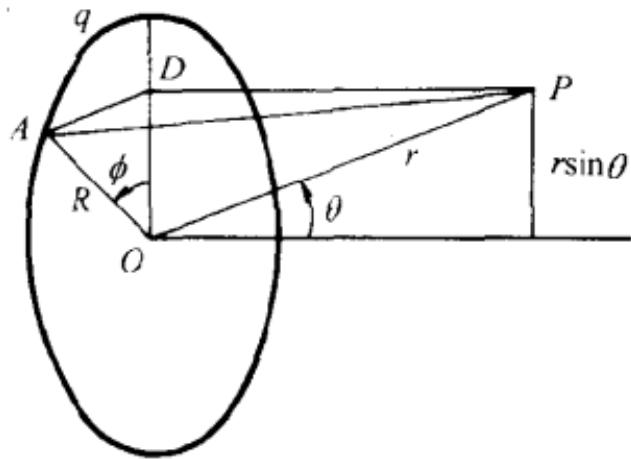
\includegraphics[width=0.5\linewidth]{figures/fig_1_4_44_2.jpg}
\end{center}

\vfill

\newpage

\textbf{1.4.45.} 两个共轴线的均匀带电圆环, 半径都是 R, 相距为 l, 所带电荷量分别为 q 和 -q. 以两环间轴线的中点 O 为原点, 沿轴线取 x 轴, 如图 1.4.45 所示. 已知 $l \ll R$ , 试求轴线上 x 处的电势.

\vfill

\textbf{1.4.46.} 半径为 R 的圆面上均匀带电, 电荷量的面密度为 $\sigma$ . 试求轴线上离圆心为 r 处的电势 U, 并由 U 求电场强度 E.

\vfill

\newpage

\textbf{1.4.47.} 两个均匀带电的圆面共轴线, 半径都是 R, 相距为 l, 电荷量的面密度分别为 $\sigma$ 和 $-\sigma$ . 以它们间轴线的中点为原点 O, 沿轴线取 x 轴, 如图 1.4.47 (1) 所示. 已知 $l \ll R$ , 试求轴线上 x 处的 (1) 电场强度 E 和 (2) 电势 U.

图1.4.47(1)

图1.4.47(2)
\begin{center}
    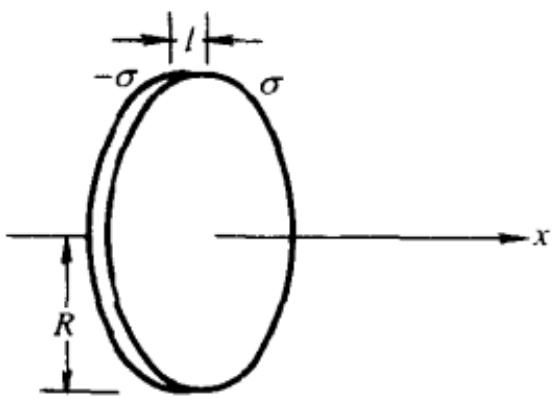
\includegraphics[width=0.5\linewidth]{figures/fig_1_4_47_1.jpg}
\end{center}
\begin{center}
    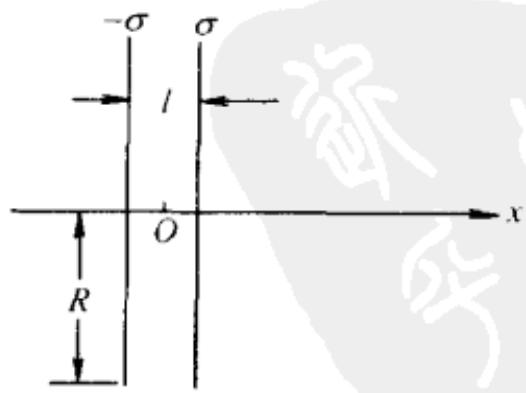
\includegraphics[width=0.5\linewidth]{figures/fig_1_4_47_2.jpg}
\end{center}

\vfill

\textbf{1.4.48.} 电荷均匀分布在半径为 R 的圆面上, 电荷量的面密度为 $\sigma$ . 试求这

图1.4.48

圆面边缘的电势.
\begin{center}
    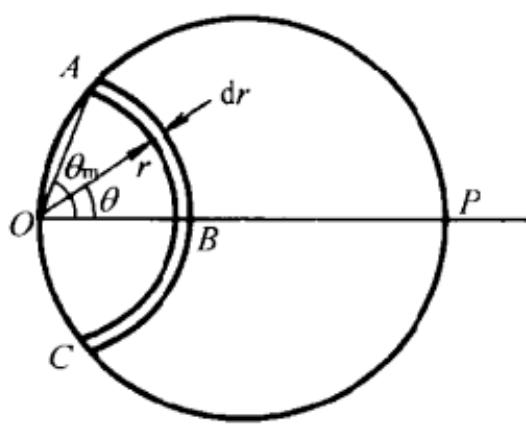
\includegraphics[width=0.5\linewidth]{figures/fig_1_4_48.jpg}
\end{center}

\vfill

\newpage

\textbf{1.4.49.} 电荷量 q 均匀地分布在半径为 R 的球面上。(1)试求离球心为 r 处的电势 U，并由 U 求电场强度 E；(2)试求离球心为 r 处的电场强度 E，并由 E 求电势 U；(3)以 r 为横坐标，U 为纵坐标，画出 U-r 曲线。

\vfill

\textbf{1.4.50.} 电荷均匀地分布在半径为 R 的球冠(球缺)面上，电荷量的面密度为 $\sigma$ ，球冠边缘对球心 O 的张角为 $2\theta$ ，如图 1.4.50 所示。试求球心 O 的电势。

\vfill

\newpage

\textbf{1.4.51.} 电荷量 q 均匀地分布在半径为 R 的半球面上. 试论证: 这半球的底面上每一点的电势都是 $\frac{q}{4\pi\varepsilon_{0}R}$ .

【论证】对于均匀分布的球面电荷，由对称性和高斯定理得出，球内处处电势相等。设想这球面分为两个半球面，由对称性可知，每个半球面上的电荷在它们的公共底面上任何两点 $A, B$ 产生的电势 $U_A$ 和 $U_B$ 必定相等。因为若 $U_A \neq U_B$ ，则两个半球面合起来成为一个球面时， $A, B$ 两点的电势便不可能相等。因此，我们得出结论：每个半球面上的电荷在其底面上任何一点所产生的电势都相等。由于半球面上的电荷量 $q$ 在球心产生的电势为 $\frac{q}{4\pi\varepsilon_0R}$ ，故得半球底面上每一点的电势都是 $\frac{q}{4\pi\varepsilon_0R}$ 。

\vfill

\textbf{1.4.52.} 电荷均匀分布在半球面上,你能否用对称性和叠加原理论证,这半球的底面上每点的电场强度都与底面垂直?

【论证】根据前面1.4.51题的结论，电荷均匀分布在半球面上，这半球面的底面便是一个等势面。因为电场强度垂直于等势面，所以均匀带电的半球面的底面上每一点，电场强度都与底面垂直。

\vfill

\newpage

\textbf{1.4.53.} 半径分别为 $R_{1}$ 和 $R_{2}$ 的两个半球面都均匀带电，电荷量的面密度分别为 $\sigma_{1}$ 和 $\sigma_{2}$ ; 这两个半球面的底面重合，球心也重合，如图 1.4.53 所示. 试求公

图1.4.53

共底面上离球心为 r 处的电势.
\begin{center}
    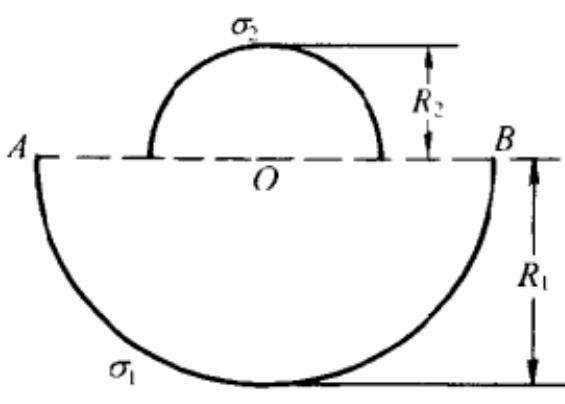
\includegraphics[width=0.5\linewidth]{figures/fig_1_4_53.jpg}
\end{center}

\vfill

\textbf{1.4.54.} 电荷均匀分布在边长为 a 的正方形平面上, 电荷量的面密度为 $\sigma$ . 试求这正方形中心的电势.

\vfill

\newpage

\textbf{1.4.55.} 一球壳体的内外半径分别为 $R_{1}$ 和 $R_{2}$ , 电荷均匀地分布在壳体内, 电荷量密度为 $\rho$ , 如图 1.4.55 所示. (1) 试求离球心为 $r$ 处的电势 $U$ ; (2) 以 $r$ 为横坐标, $U$ 为纵坐标, 画出 $U - r$ 曲线.

\vfill

\textbf{1.4.56.} 电荷量 q 均匀地分布在半径为 R 的球体内。(1)试求离球心为 r 处的电势 U; (2)以 r 为横坐标, U 为纵坐标, 画出 U-r 曲线.

\vfill

\newpage

\textbf{1.4.57.} 氢原子处在基态时,核外电荷分布如下:在距离核为 r 处,电荷量密度为 $\rho(r)=-\frac{q}{\pi a^{3}}\mathrm{e}^{-\frac{2r}{a}}$ , 式中 q 是电子电荷量的大小, a 是玻尔半径. 试求 r 处(1)核外电荷所产生的电势; (2)所有电荷产生的电势.

\vfill

\textbf{1.4.58.} 两个均匀带电的无限长直共轴圆筒,内筒半径为 a,沿轴线单位长度的电荷量为 $\lambda$ ,外筒半径为 b,沿轴线单位长度的电荷量为 $-\lambda$ .试求:(1)离轴线为 r 处的电势;(2)两筒的电势差.

\vfill

\newpage

\textbf{1.4.59.} 两个长直圆筒共轴,它们的半径分别为1.5cm和3.0cm,两筒面上都均匀带电,沿轴线单位长度的电荷量大小相等而符号相反,已知它们的电势差为5000V.试问何处电场强度最大?其值是多少?

\vfill

\textbf{1.4.60.} 根据电场强度 E 与电势 U 的关系 E = -VU，试由下列三种情况的 U 求相应的 E：(1) 点电荷 q: $U = \frac{q}{4\pi\varepsilon_{0}} \frac{1}{r}$ ; (2) 圆环电荷 q 的轴线上: $U = \frac{q}{4\pi\varepsilon_{0}} \times \frac{1}{\sqrt{r^{2} - R^{2}}}$ ，式中 R 是圆环半径，r 是到环心的距离；(3) 电偶极子 p: $U = \frac{p}{4\pi\varepsilon_{0}} \times \frac{\cos\theta}{r^{2}}$ .

\vfill

\newpage
